%% LyX 1.3 created this file.  For more info, see http://www.lyx.org/.
%% Do not edit unless you really know what you are doing.
\documentclass[12pt,letterpaper,english]{scrbook}
\usepackage{times}
\usepackage[T1]{fontenc}
\usepackage[latin1]{inputenc}
\setcounter{secnumdepth}{3}
\setcounter{tocdepth}{3}
\usepackage{array}
\usepackage{longtable}
\usepackage{varioref}
\usepackage{color}
\usepackage{graphicx}

\makeatletter

%%%%%%%%%%%%%%%%%%%%%%%%%%%%%% LyX specific LaTeX commands.
\newcommand{\noun}[1]{\textsc{#1}}
%% Bold symbol macro for standard LaTeX users
\providecommand{\boldsymbol}[1]{\mbox{\boldmath $#1$}}

%% Because html converters don't know tabularnewline
\providecommand{\tabularnewline}{\\}

%%%%%%%%%%%%%%%%%%%%%%%%%%%%%% Textclass specific LaTeX commands.
 \usepackage{verbatim}

%%%%%%%%%%%%%%%%%%%%%%%%%%%%%% User specified LaTeX commands.
\usepackage{babel}
\usepackage{longtable}
\usepackage{color}
\usepackage{graphicx}
\usepackage{html}
\usepackage{hyperref} 
\newcommand{\pjal}{\emph{JAL 2.0}}
\parskip=0.5em
\widowpenalty=10000
\clubpenalty=10000
\raggedbottom

\usepackage{babel}
\makeatother
\begin{document}

\title{\pjal\ manual}


\author{\noun{Javier Mart�nez} \and \noun{Dave Lagzdin} \and \noun{Vasile
Surducan}}


\lowertitleback{\pjal\ \textcolor{black}{Manual}\\
\textcolor{black}{}\\
\textcolor{black}{Copyright \copyright  2006} \textcolor{black}{\noun{Javier
Mart�nez}}\textcolor{black}{,} \textcolor{black}{\noun{Dave Lagzdin}}
\textcolor{black}{~and}\textcolor{black}{\noun{~Vasile Surducan}}\textcolor{black}{.
}\\
\textcolor{black}{}\\
\textcolor{black}{Permission is granted to copy, distribute and/or
modify this document under the terms of the GNU Free Documentation
License, Version 1.2 or any later version published by the Free Software
Foundation; with no Invariant Sections,} with this Front-Cover \textcolor{black}{Texts,
and no Back-Cover Texts. A copy of the license is included in the
section entitled ''GNU Free Documentation License''.} }

\maketitle
\begin{comment}
Update pJAL name in Preamble!!
\end{comment}

\chapter*{\pjal\ manual}

\pjal\ \cite{pJALdownload} is a high-level language for a number
of Microchip \texttrademark~PIC microcontrollers~\cite{Microchip-web}.

It was created by \noun{Kyle York}, who also wrote the \emph{PICbsc}
compiler~\cite{PICbsc}. \noun{Stef Mientki} got in touch with
\noun{Kyle York} and ask him if he could look into rewriting \emph{JAL}
using the \emph{PICbsc} engine, the prospect intrigued him\emph{.}
\pjal\ not only shares the same \emph{JAL~\cite{Wouter-web}} syntax,
but adds new features (like new types, arrays, etc.) to \emph{JAL,}
keeping the \emph{PICbsc} internal compiler design as well. This manual
covers all aspects of \pjal\ without any reference to \emph{JAL}
trying to be useful for all, novices and users with \emph{JAL} experience. 

\emph{JAL} was developed by \noun{Wouter van Ooijen}%
\footnote{Wouter released JAL under GPL (\htmladdnormallink{http://jal.sourceforge.net}{http://jal.sourceforge.net})
in January of 2003.%
}. He created \emph{JAL} because he did not like any of the low-cost
(or free) languages for these chips and implementing a high level
language looked like a nice project. 

For a quick impression of \pjal\ here's a small example how \pjal\
looks. Also, you could read either the summary%
\footnote{See section \ref{sec:GNU-FDL}~\vpageref{sec:GNU-FDL}%
} or the examples%
\footnote{See section \ref{sec:Examples}~\vpageref{sec:Examples}%
} section of this manual.

\textbf{Example}:\\
\begin{verbatim} 
   ; microcontroller definition file
   include c16F877_10

   ; set pin a0 direction as output
   pin_a0_direction = output 

   ; do forever the statements inside the loop
   forever loop 
 
     pin_a0 = ! pin_a0  ; complement value of a0
     delay_1s(1)        ; wait 1 second
 
   end loop
   
\end{verbatim}

\tableofcontents{}


\newpage
\chapter*{Revision history}

\label{sec:Revision-history}

\begin{description}
\item [7th~March~2006]First edition, \emph{pJAL} version 0.9 (Released
on 2006 March 2).\\
{\small Written by:} \noun{\small Javier Mart�nez, Dave Lagzdin}
{\small and} \noun{\small Vasile Surducan}\\
{\small Thanks to:} \noun{\small Joep Suijs, Kyle York}{\small ,}
\noun{\small Michael Watterson, Stef Mientki} {\small and} \noun{\small Wouter
van Ooijen.}{\small \par}
\item [21th~April~2006]Second edition, \emph{JAL} 2.0 (Released on 2006
April 20).\\
{\small Updated by:} \noun{\small Javier Mart�nez, Dave Lagzdin}
{\small and} \noun{\small Vasile Surducan}{\small }\\
{\small Modifications: changed compiler name, corrected small} \emph{\small bugs,}
{\small added some suggestions and updated multi-word configuration
bits.}{\small \par}
\item [10th~June~2006]Third edition, \emph{JAL 2.0} (Released on 2006
June 8).\\
{\small Updated by:} \noun{\small Javier Mart�nez, Dave Lagzdin}
{\small and} \noun{\small Vasile Surducan}{\small }\\
{\small Thanks to:} \noun{\small Norbert Schlichthaerle, Andree
Steenveld.}{\small }\\
{\small Modifications: corrected small} \emph{\small bugs,} {\small added
some suggestions and new compiler features.}{\small \par}
\end{description}

\newpage
\chapter{Language definition}

\label{sec:Language-definition}


\section{basics}

\label{sub:Language-basics}\htmlrule


\subsection{Format}

\label{sub:Format}

The \pjal\ language is free-format (except for comments) and not
case-sensitive. All characters with an ASCII value below the space
(tab, carriage return, new line, form feed, etc.) are treated as spaces,
except that the end of a line terminates a comment.

\pjal\ does not use statement separators. The only real separators
are the comma's between the (formal or actual) arguments to a procedure
or function \verb+"( , )"+, or in an array definition \verb+"{ , }"+.

\begin{comment}
The \emph{pJAL} syntax is based on tokens. Tokens must be separated
by separators, hence spaces (or other separators) are needed between
identifiers, operators etc. 
\end{comment}
\textbf{Example}:\\
\begin{verbatim} 
   -- if statement in preferred format
   if a > b then
      a = b + 1
   else
      a = b - 1
   end if
    
   -- but this has exactly the same effect
   if a > b then a = b + 1 else a = b - 1 end if
   
   -- comma's between actual arguments
   f( a, b, c, d )
   var byte msg[5] = "Hello"
   
\end{verbatim}

\htmlrule


\subsection{Comments}

\label{sub:Comments}

A comment is started by the token \verb+"--"+ or \verb+";"+ and
continues until the end of the line.\\
\\


\textbf{Example}: \begin{verbatim}   -- the next line contains a comment 
   -- after the assignment
   ticks = ticks + 1 ; one more tick
    
   ; the next line contains the same comment 
   ; after the assignment
   ticks = ticks + 1 -- one more tick
   
\end{verbatim}

\htmlrule


\subsection{Includes }

\label{sub:Includes}

An include causes the content of the included file to be read. A subsequent
include for the same file name will be ignored. This makes it possible
for a library file to include all required lower libraries.

Included files are sought first in the current directory, and next
in each location indicated by the compilers search path. All \emph{}\pjal\
files have the extension \verb+".jal"+. Be care not to include this
extension in the \emph{include} statement.

Includes can be nested to any level.

\textbf{Example}:\\
\begin{verbatim} 
   include serial    -- include the serial.jal file
   include i2c       -- include the i2c.jal file
   
\end{verbatim}

\htmlrule


\subsection{Program}

A \pjal\ program is a sequence of statements. Declarations are also
considered statements, so declarations can appear almost anywhere
in a program.

\textbf{Example}:\\
\begin{verbatim} 
   -- my first program 
   var byte b       -- variable declaration
   while b > 0 loop -- start of loop
      b = b + 1     -- variable assignment
   end loop         -- end of loop
   
\end{verbatim}

\htmlrule


\subsection{Scope}

\pjal\ is a block-structured language, so each declaration is visible
from its declaration to the end of the block in which the declaration
appears (in practice this means to the first end at the current nesting
level).

A declaration can hide a declaration of the same name from an enclosing
block. A declaration can not hide a name which was already declared
at the same nesting level.

\textbf{Example}:\\
\begin{verbatim} 
   var byte b
   while b > 0 loop
      var bit b    -- Overrides the byte b defined
                   -- outside the while block.
   
      b = false    -- The bit b, not the byte
   
      var byte b   -- Error, "b" already declared
                   -- as a bit inside the while block.
   end loop
   
   var word b      -- Error, "b" already declared
                   -- as a byte before while block.
   
\end{verbatim}

\htmlrule


\subsection{Block}

A block is a sequence of statements. Variables, constants, procedures,
and functions defined in a block will not be visible outside of the
block.


\section{basic types}

\label{sub:basic-types}\htmlrule


\subsection{Built-in types}

\label{sub:Built-in-types}These are the types of range values that
\pjal\ supports.

\begin{description}
\item [BIT]1 bit unsigned boolean value (range is 0 or 1)%
\footnote{ \pjal\ support aditional names for this range: \emph{0 = FALSE =
LOW = OFF} and \emph{1=TRUE=HIGH=ON.}%
}.
\item [BYTE]8 bit unsigned value (range is 0 .. 255).
\item [SBYTE]8 bit signed value (range is -128 .. 127).
\item [WORD]16 bit unsigned value (range is 0 .. 65,535).
\item [SWORD]16 bit signed value (range is -32,768 .. 32,767).
\item [DWORD]32 bit unsigned value (range is 0 .. 4,294,967,296).
\item [SDWORD]32 bit signed value (range is -2,147,483,648 .. 2,147,483,647).
\item [\htmlrule]~
\end{description}

\subsection{Extending types}

\label{sub:Extending-types-with}Basic types can be extended using
the token \emph{{[}{*}cexpr{]}}%
\footnote{\emph{cexpr} means a constant expression or a literal value.%
} preceded by token \emph{type}. Being \emph{type} one of the following
built-in types%
\footnote{See section \ref{sub:Built-in-types}~\vpageref{sub:Built-in-types}%
}: BIT, BYTE or SBYTE.

\html{\\}


\paragraph{\emph{BYTE} and \emph{SBYTE}\protect \\
}

For \emph{BYTE} and \emph{SBYTE}, this means the variable will be
defined as an integer using \emph{cexpr} bytes.

\textbf{Example}: \begin{verbatim}    WORD is simply shorthand for BYTE*2 
   DWORD is simply shorthand for BYTE*4 
\end{verbatim}\html{\\}


\paragraph{BIT\protect \\
}

If type is \emph{BIT}, the definition changes. A \emph{BIT} variable,
as defined in \emph{JAL}, is really of type boolean. When assigned
any non-zero value, it takes on the value of 1.

Using the \emph{{[}}{*}cexpr\emph{{]}}, the definition changes to
be more like a C bit field: assignment is masked.

We can create a 'nibble-like' grouping of bits with range 0 to ($2^{cexpr}-1$),
i.e.: with 2 bits we can count to 3 ( 0b11 ) 

\textbf{Example}: \begin{verbatim}    VAR BIT*2 cc 
   
   -- when assigning to cc, the internal 
   -- compiler assignment is: 
   cc = (value & 0x03) -- mask 2 least significative bits
                       -- remember 0x03=0b00000011
   
\end{verbatim}


\section{Literals}

\label{sub:Literals} Literals are numeric constants with a invariant
value, the format is:

\begin{description}
\item [12]a decimal numeric constant
\item [0x12]a hexadecimal numeric constant
\item [0b01]a binary numeric constant
\item [0q01]an octal numeric constant
\item [\char`\"{}a\char`\"{}]an ASCII char constant
\item [\char`\"{}Hello\char`\"{}]a \emph{string} constant. Following \emph{escape
sequence} chars can be used inside a string:\\
\\
\begin{tabular}{|c|l|}
\hline 
Escape sequence char&
Description\tabularnewline
\hline
\hline 
\verb+\a+&
Bell\tabularnewline
\hline 
\verb+\b+&
Backspace\tabularnewline
\hline 
\verb+\f+&
Form Feed\tabularnewline
\hline 
\verb+\n+&
Line Feed\tabularnewline
\hline 
\verb+\r+&
Carriage Return\tabularnewline
\hline 
\verb+\t+&
Horizontal TAB\tabularnewline
\hline 
\verb+\v+&
Vertical TAB\tabularnewline
\hline 
\verb+\\+&
\textbackslash{}\tabularnewline
\hline 
\verb+\?+&
?\tabularnewline
\hline 
\verb+\'+&
'\tabularnewline
\hline 
\verb+\"+&
''\tabularnewline
\hline 
\verb+\0+&
Hexadecimal value: \verb+0x00+\tabularnewline
\hline 
\verb+\x##+&
Hexadecimal value: \verb+0x##+\tabularnewline
\hline
\end{tabular}
\end{description}
Literals other than ASCII constants may also contain a number of underscores
\verb+"_"+ which are ignored, but are useful for making them more
readable.

\textbf{Example}: \begin{verbatim}    0b_0000_1111  -- a binary literal
   
   -- a fuse definition (14 bit word)
   0b_11_0000_1111_0000 
   
   1_234_567     -- a decimal literal
   
\end{verbatim}

String constants can use C style initialization style, eg:

\verb+var byte string[] = "abc" "def" "ghi"+

is the same as:

\verb+var byte string[] = "abcdefghi"+


\section{Constants}

\label{sub:Constants}A constant declaration introduces a name which
has a constant value throughout its scope. When the type is omitted
the constant has a \emph{SDWORD} type. A single constant declaration
can introduce a number of constants of the same type.

\begin{verbatim} 
   CONST [type[*cexpr]] identifier [ '[' cexpr ']' ]

   { '=' cexpr | = '{' cexpr1[, cexpr2,...]'}' | = '"' cexpr '"'}

   [ , identifier2...]
   
\end{verbatim}

\html{\\}

\begin{description}
\item [CONST]denotes the beginning of a constant definition clause.
\end{description}
\html{\\}

\begin{description}
\item [type{[}{*}cexpr{]}]Defines the type of the constant. If none is
given, the constant becomes universal type which is 32 bit signed
(\emph{SDWORD}).
\end{description}
\html{\\}

\begin{description}
\item ['{[}'~cexpr~'{]}']Defines a constant table %
\footnote{See section \ref{sub:Constant-tables}~\vpageref{sub:Constant-tables}%
}.\\
A constant table will not take any space unless it is indexed at least
once with a non-constant subscript. On the PIC, constant tables consume
\emph{code} space, not \emph{data} space, and are limited to 255 elements. 
\end{description}
\html{\\}

\begin{description}
\item ['='~cexpr]For non-table constants this assigns the value to the
constant.
\end{description}
\html{\\}

\begin{description}
\item ['='~'\{'~cexpr1{[},~cexpr2~\ldots{]}~'\}']For tables of constants
this assigns the value to each element. There must be the same number
of \emph{cexprs} as there are elements defined. 
\item [\html{\\}]~
\item [''''~cexpr~'''']A \emph{string} constant can be assigned to
a constant table: \\
\verb+const byte x[] = "hello"+.
\end{description}
\html{\\}

\textbf{Example}: \begin{verbatim}    const byte cr = 0x0D, lf = 10 -- byte constants
   const word cr = 1492          -- word constant
   
   -- Literal (SDWORD) constant
   const seconds_per_day = 60 * 60 * 24
   
   -- constant table
   const byte mytable[5] = {"M","2",24,1,43} 
   -- String constant table
   const byte zz[] = "Hello"
   
   -- Extended type constant
   const byte*3 my_pointer = 0xFFCC00
   
\end{verbatim}


\section{Variables}

\label{sub:Variables}


\subsection{Declaration}

\label{sub:Variable-Declaration}

A variable declaration introduces a name which will be used within
the \pjal\ program. In PIC architecture this name will correspond
to a hardware location called \emph{register} located in RAM memory. 

These \emph{registers} can be of two types: 

\begin{itemize}
\item GPR. General Purpose Registers
\item SFR. Special Function Registers
\end{itemize}
Optionally the name can be bound to a specific location%
\footnote{See section \ref{sub:Location}~\vpageref{sub:Location}%
}, or to other already declared variable%
\footnote{See section \ref{sub:Alias}~\vpageref{sub:Alias}%
}, otherwise the compiler allocates a suitable and available GPR location. 

In a declaration a value can be assigned to a variable, which has
the same effect as an equivalent assignment immediately following
the declaration. 

\textbf{Example}: \begin{verbatim}    var byte demo = 0xAF 
   
   --  ... same as ...
   var byte demo
   demo = 0xAF
   
\end{verbatim}

The initial value does not need to be a constant expression.

\pjal\ will set the correct bank memory while addressing a variable
(except in inline assembler%
\footnote{See section \ref{sub:Inline-assembler}~\vpageref{sub:Inline-assembler}%
}).

\begin{verbatim}    VAR [VOLATILE] type[*cexpr] 
      identifier [ '[' cexpr ']' ]

      [ { AT cexpr [ : bit ] | 
             variable [ : bit ] | 
            '{' cexpr1[, cexpr2...] '}'

      | IS variable }

    [ '=' cexpr | '{' cexpr1, ... '}' | '=' '"' cexpr '"']

    [, identifier2...]

\end{verbatim}

\html{\\}

\begin{description}
\item [VAR]denotes the beginning of a variable definition clause.
\end{description}
\html{\\}

\begin{description}
\item [VOLATILE]A variable can be declared volatile, which expresses that
the variable does not possess normal variable semantics%
\footnote{See section \ref{sub:Volatile}~\vpageref{sub:Volatile}%
}. 
\end{description}
\html{\\}

\begin{description}
\item [type{[}{*}cexpr{]}]The \emph{type} of the variable%
\footnote{See section \ref{sub:Built-in-types}~\vpageref{sub:Built-in-types}
and section \ref{sub:Extending-types-with}~\vpageref{sub:Extending-types-with}.%
}. 
\end{description}
\html{\\}

\begin{description}
\item [Identifier]Any valid \pjal\ identifier.
\end{description}
\html{\\}

\begin{description}
\item ['{[}'~cexpr~'{]}']Defines a table%
\footnote{See section \ref{sub:Variable-tables}~\vpageref{sub:Variable-tables}.%
} of \emph{cexpr}%
\footnote{\emph{cexpr} means a constant expression or a literal value.%
} elements. The table index starts at 0 and continues through (cexpr
- 1). cexpr must be >= 1. A table \emph{MUST} fit entirely within
a single PIC data bank.
\end{description}
\html{\\}

\begin{description}
\item [AT~\ldots]denotes the location of the variable%
\footnote{See section \ref{sub:Location}~\vpageref{sub:Location}%
}. 
\end{description}
\html{\\}

\begin{description}
\item [IS~variable]Tells the compiler that this identifier is simply an
alias for another%
\footnote{See section \ref{sub:Alias}~\vpageref{sub:Alias}%
}. 
\end{description}
\html{\\}

\begin{description}
\item ['='~expr]Shorthand assignment. The variable will be assigned expr.
\end{description}
\html{\\}

\begin{description}
\item ['='~'\{'~expr1~{[},~expr2~\ldots{]}~'\}']For a table variable,
the elements will be assigned expr1, expr2, \ldots. 
\end{description}
\html{\\}

\begin{description}
\item [''''~cexpr~'''']A \emph{string} constant can be assigned to
a variable table: \\
\verb+var byte x[5] = "hello"+.
\end{description}
\html{\\}

\begin{description}
\item [,~identifier2~\ldots]Allows defining multiple variables with
the same attributes: VAR BYTE a,b,c
\end{description}
\html{\\}

\begin{verbatim}    var byte x, y=3
   var word z
   var dword i=0
   var byte AD_lo, AD_hi
   var word AD_result = AD_lo + 256*AD_hi
   
\end{verbatim}

\htmlrule


\subsection{Location}

\label{sub:Location}

A variable declaration can specify the adress of the variable. The
address expression must be compile-time constant. The compiler takes
care of the translation to the banked address. 

\begin{description}
\item [AT~cexpr~{[}~':'~bit~{]}]Places the new variable at address
\emph{cexpr}. 
\end{description}
\html{\\}

\begin{description}
\item [AT~variable~{[}~':'~bit~{]}]Places the new variable at the
same address as an existing variable. Any address uses for explicit
placement will not be allocated to another variable.
\end{description}
\html{\\}

\begin{description}
\item [AT~'\{'~cexpr1{[},~cexpr2~\ldots{]}~'\}']Places the new variable
at multiple address. On the PIC, many of the special purpose registers%
\footnote{SFRs in Microchip\texttrademark's terminology.%
} are mirrored in two or more data banks. Telling the compiler which
address hold the variable allows it to optimize the data access bits.
\end{description}
\html{\\}

\begin{verbatim}   var byte volatile porta at 0x06
   var volatile byte _status AT {0x0003, 0x0083, 
                                 0x0103, 0x0183}
   var bit  volatile _z at _status : 2
   
\end{verbatim}

\htmlrule


\subsection{Volatile}

\label{sub:Volatile}

The \emph{VOLATILE} keyword guarantees that a variable that is either
used or assigned will not be optimized away, and the variable will
be only read once when evaluating an expression. Normally, if a variable
is assigned a value that is never used, the assignment is removed
and the variable will not allocated any space.

If the assignment is an expression, the expression \emph{will} be
fully evaluated. If a variable is used, but never assigned, all instances
of the variable \emph{will} be replaced with the constant 0 (of the
appropriate type) and the variable \emph{will not} be allocated any
space.

SFR's should always be declared as \emph{VOLATILE}, as these are associated
with certain hardware functions specific to the PIC being used. 

\begin{verbatim}   var volatile byte FSR at 4 
   var volatile byte INDF at 0
   var volatile byte count
   
\end{verbatim}

\htmlrule


\subsection{Alias}

\label{sub:Alias}

A variable can be declared to be an alias for another variable. This
is used much like a constant declaration to hide the actual identity
of an identifier from subsequent code.

\begin{verbatim}   -- fragment of a library file,
   -- which defines the pins used by the library
   var byte volatile i2c_clock    is pin_a3
   var byte volatile i2c_data_in  is pin_a4
   var byte volatile i2c_data_out is pin_a4_direction
   
\end{verbatim}


\section{Tables}

\label{sub:Tables}


\subsection{Constant tables}

\label{sub:Constant-tables}

Constant tables are stored in program code, they're limited to 255
values.

\begin{verbatim}   const byte msg[5] = {"M","2",24,1,43} 
\end{verbatim}

A constant table will produce no code unless it's used with a variable
subscript. So, if you use: 

\begin{verbatim}   -- Constant index:
   -- "msg[3]" will replace by the corresponding
   -- literal value, like: a=1
   a = msg[3] 
\end{verbatim}

\ldots~the constant value \emph{1} will be assigned into variable
\emph{a}. And if you use: 

\begin{verbatim}   -- Variable index:
   -- A special look up table function is built 
   x = 3
   a = msg[x]
\end{verbatim}

\ldots\emph{~msg} will become a lookup table function that will
return the desired value.

If constant table is declared with values assignment, it's not necessary
to include the table \emph{index:}

\begin{verbatim}   const byte msg[] = {"M","2",24,1,43} 
\end{verbatim}

In order to know the amount of values in the table you must use the
COUNT statement%
\footnote{See section \ref{sub:COUNT}~\vpageref{sub:COUNT}%
}.


\subsection{Variable tables}

\label{sub:Variable-tables}

Variable tables are stored in RAM memory and must fit within a single
bank.

\begin{verbatim}   var byte msg[5] = {"M","2",24,1,43} 
\end{verbatim}

\begin{enumerate}
\item when \emph{defining} a table, the size must be const, so\\
var byte myvar{[}3{]} ; this is valid\\
var byte myvar{[}n{]} ; this is \emph{NOT} valid if \emph{n} is a
variable
\item when \emph{using} the table, the index can be either const or a variable.
The table starts at index 0. When using a variable, no bounds checking
is done.
\end{enumerate}
\begin{verbatim}   -- Constant index:
   -- "msg[3]" will replace by the exact file register
   -- with the index 3
   a = msg[3] 
   
   -- Variable index:
   -- An INDIRECT MEMORY ACCESS is used to get the value
   x = 3
   a = msg[x]
\end{verbatim}

If variable table is declared with values assignment, it's not necessary
to include the table \emph{index:}

\begin{verbatim}   var byte msg[] = "Hello" 
\end{verbatim}

In order to know the amount of values in the table you must use the
COUNT statement%
\footnote{See section \ref{sub:COUNT}~\vpageref{sub:COUNT}%
}.


\section{Expressions}

\label{sub:Expressions}

An expression is constructed from literals, identifiers, function
calls and operators. An identifier can identify a constant, a variable
or (within a subprogram) a formal parameter.

\htmlrule


\subsection{Operators}

\label{sub:Operators}The following operators are defined in \pjal\
(ordered by priority):

\html{\\}

\medskip{}
\begin{center}\begin{longtable}{|c|l|c|>{\raggedright}p{6cm}|}
\hline
\hline 
\textbf{Op.}&
\textbf{Description}&
\textbf{Priority}&
\textbf{Example}\tabularnewline
\hline
\endhead
\hline
\hline 
\textbf{Op.}&
\textbf{Description}&
\textbf{Priority}&
\textbf{Example}\tabularnewline
\hline
\hline
\endfirsthead
\hline
\hline 
\multicolumn{4}{|c|}{\ldots}\tabularnewline
\hline
\endfoot
\hline
\hline 
\multicolumn{4}{|c|}{}\tabularnewline
\hline
\hline
\endlastfoot
\hline 
\verb+!!+&
Logical&
0 (highest)&
\verb+!!5 = 1 +\newline\verb+!!0 = 0+\tabularnewline
\hline 
\verb+-+&
Unary negation&
0 (highest)&
\verb+-1 -- negative+\tabularnewline
\hline 
\verb+!+&
Bitwise complement&
0 (highest)&
\verb+var byte a=0b_0000_1111+\newline\verb+a=!a+\newline\verb+-- a=0b_1111_0000 +\tabularnewline
\hline 
\verb+~+&
Bitwise complement&
0 (highest)&
\verb+var byte a=0b_0000_1111+\newline\verb+a=~a+\newline\verb+-- a=0b_1111_0000 +\tabularnewline
\hline 
\verb+*+&
Multiplication&
1&
\verb+var byte a = 2+\newline\verb+a=a*3 -- a=6+\tabularnewline
\hline 
\verb+/+&
Integer division&
1&
\verb+var byte a = 17+\newline\verb+a=a/2 -- a=8+\tabularnewline
\hline 
\verb+%+&
Modulus division&
1&
\verb+var byte a = 17+\newline\verb+a=a%2 -- a=1+\tabularnewline
\hline 
+&
Addition&
2&
\verb+var byte a = 2+\newline\verb+a=a++\verb+3 -- a=5+\tabularnewline
\hline 
\verb+-+&
Subtraction&
2&
\verb+var byte a = 17+\newline\verb+a=a-10 -- a=7+\tabularnewline
\hline 
\verb+<<+&
Left shift&
3&
\verb+var byte a = 0x81+\newline\verb+a=a<<1 -- a=0x02+\tabularnewline
\hline 
\verb+>>+&
Right shift&
3&
\verb+var byte a = 0x82+\newline\verb+a=a>>1 -- a=0x41+\tabularnewline
\hline 
\verb+<+&
Less than&
3&
\verb+var byte a=12, b=14+\newline\verb+if a < b then ...+\tabularnewline
\hline 
\verb+<+\verb+=+&
Less or equal than&
3&
\verb+var byte a=12, b=12+\newline\verb+if a <= b then ...+\tabularnewline
\hline 
\verb+==+&
Equal&
3&
\verb+var byte a=12, b=12+\newline\verb+if a == b then ...+\tabularnewline
\hline 
\verb+!+\verb+=+&
Not equal&
3&
\verb+var byte a=12, b=14+\newline\verb+if a != b then ...+\tabularnewline
\hline 
\verb+>+\verb+=+&
Greater or equal than&
3&
\verb+var byte a=14, b=12+\newline\verb+if a >= b then ...+\tabularnewline
\hline 
\verb+>+&
Greater than&
3&
\verb+var byte a=12, b=12+\newline\verb+if a >= b then ...+\tabularnewline
\hline 
\verb+&+&
Bitwise AND&
4 (lowest)&
\verb+var byte a=0b_1111_1110+\newline\verb+a=a&0b_0000_0011+\newline\verb+-- a=0b_0000_0010 +\tabularnewline
\hline 
\verb+|+&
Bitwise OR&
4 (lowest)&
\verb+var byte a=0b_0000_1110+\newline\verb+a=a|0b_0011_1100+\newline\verb+-- a=0b_0011_1110 +\tabularnewline
\hline 
\verb+^+&
Bitwise XOR&
4 (lowest)&
\verb+var byte a=0b_1111_1110+\newline\verb+a=a^0b_0000_0011+\newline\verb+-- a=0b_1111_1101 +\tabularnewline
\end{longtable}\end{center}

Tips:

\begin{itemize}
\item The \emph{Logical} operator \verb+"!!"+ returns 0 if the operand
is 0, or 1 if the operand is not 0. It's useful in some expressions
which need a guarantee that operand is either 1 or 0.
\item Right shift is logical for unsigned types, and arithmetic for signed
types (it's sign preserving). 
\end{itemize}
\smallskip{}
\begin{center}Logical right shift (for unsigned types):\end{center}

\begin{center}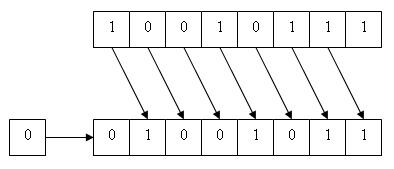
\includegraphics[%
  clip]{LogicalShiftRight.png}\end{center}

\smallskip{}
\begin{center}Arithmetic right shift (for signed types):\end{center}

\begin{center}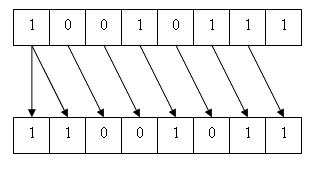
\includegraphics[%
  clip]{ArithmaticShiftRight.png}\end{center}

\begin{itemize}
\item Operands to binary operations \emph{MUST} be the same, and return
the type of the operand \emph{EXCEPT} the relationals (\verb+">="+,
\verb+"<"+, etc.), which return a BIT value. 
\end{itemize}
\textbf{Example}: \begin{verbatim}   -- Use of relationals as BIT type selector:
  const myclk = 1 * ( SPI_clock == (target_clock / 4)  ) +
                2 * ( SPI_clock == (target_clock / 16) ) +
                3 * ( SPI_clock == (target_clock / 64) )
   -- myclk being assigned 1, 2, 3, or 0.
\end{verbatim}

\begin{itemize}
\item An exception to the above rule is the universal type : when used in
an expression, the universal type will be converted to type of the
other operand.
\end{itemize}
\html{\\}

\textbf{Example}: \begin{verbatim}   var byte a = 1 << n
   if ( a > b ) | ( c < d ) | ( x != y ) then 
      x = ( x & 0b_1100_0011 ) | 0b_0001_0100
   end if
\end{verbatim}

\htmlrule


\subsection{Priority}

\label{sub:Priority}

Braces can be used to force the association, otherwise the operator's
associate with their arguments according to operator's priority. 

\html{\\}

\textbf{Example}: \begin{verbatim}   var byte x = ! a + b  -- ( ! a ) + b
   var y = ! ( a + b )   -- not the same as previous
\end{verbatim}


\section{Statements}

\label{sub:Statements}A statement is any variable, constant, function,
or procedure definition, assignment, control (IF) or looping (FOR,
FOREVER, WHILE).

\htmlrule


\subsection{Declaration}

Declarations are considered statements, so declarations can appear
anywhere in a program where a statement is allowed. 

\textbf{Example}: \begin{verbatim}   a = 5
   -- need a few locals here? no problem!
   var byte x = 1, y = 0
   while x < a loop 
      y = y + x
      x = x + 1
   end loop
   
\end{verbatim}

\htmlrule


\subsection{Assignment}

An assignment statement evaluates the expression and assigns its value
to the variable or formal parameter indicated by the name on the left
of the assignment.

\textbf{Example}: \begin{verbatim}   var byte a
   procedure p( byte out q ) is 
      q = 5 -- assign to the (out) parameter q
      a = 4 -- assign to the global variable a
   end procedure 
   a = 5 -- assign to the (now local) variable a
   
\end{verbatim}

\htmlrule


\subsection{IF}

An \emph{IF} statement evaluates an expression. If the result is true
the list of statements following the \emph{THEN} token is executed.

Before the \emph{ELSE} token any number of \emph{ELSIF} tokens can
appear. When the \emph{IF} condition is false, the first \emph{ELSIF}
condition is evaluated. If it is true the corresponding statements
are executed, otherwise execution continues with the next \emph{ELSIF}
part.

When none of the \emph{IF} and \emph{ELSIF} conditions evaluate to
true the statements in the optional \emph{ELSE} part are executed. 

The IF statement serves two purposes:

\html{\\}


\paragraph{Conditional execution}

\begin{verbatim}   IF expr THEN 
      block 
   [ ELSIF expr THEN block ... ] 
   [ ELSE block ] 
   END IF
\end{verbatim}

\begin{quotation}
Note: any number of ELSIF conditions may be present.
\end{quotation}
\textbf{Example}: \begin{verbatim}   IF myvar = 13 THEN
      -- Case of myvar = 13 ... 
   ELSIF myvar = 10 THEN
      -- Case of myvar = 10 ... 
   ELSE
      -- Any other values of myvar
   END IF
\end{verbatim}\html{\\}


\paragraph{Conditional compilation}

\begin{verbatim}   IF cexpr THEN
      block 
   [ ELSIF cexpr THEN block ...] 
   [ ELSE block ] 
   END IF
\end{verbatim}

In this case, a new scope is \emph{NOT} opened. If \emph{cexpr}%
\footnote{\emph{cexpr} means a constant expression or a literal value.%
} is 0, the associated statements are skipped without further processing,
so it can be used to create a block comment.

\textbf{Example}: \begin{verbatim}   IF target_chip = 16f877 THEN
      -- Execution part if PIC16F877 
   ELSIF target_chip = 16f876 THEN
      -- Execution part if PIC16F876 
   ELSE
      -- Execution part other chips 
   END IF
\end{verbatim}\htmlrule


\subsection{WHILE}

The WHILE statement allows conditional looping.

\begin{verbatim}   WHILE expr LOOP
      block 
   END LOOP
\end{verbatim}

A while statement evaluates the expression (\emph{expr}). If the result
is false, the while statement has completed its execution. Otherwise
the statements are executed, after which the expression is evaluated
again etc. The \emph{block} statements will be executed as long as
\emph{expr} is non-0

\textbf{Example}: \begin{verbatim}   while r > y loop
      d = d + 1
      r = r - y
   end loop

\end{verbatim}

\htmlrule


\subsection{FOR}

The FOR statement allows looping a given number of times.

\begin{verbatim} 
   FOR expr [ USING variable ] LOOP 
      block 
   END LOOP
\end{verbatim}

\begin{comment}
If the \emph{IN variable} clause does not exist, this becomes:

\begin{verbatim} 
   _temp = 0 
   WHILE (_temp < expr) LOOP
      block
      _temp = _temp + 1
   END LOOP
\end{verbatim}
\end{comment}
If the \emph{USING variable} clause does not exist, the variable \emph{\_temp}
is used instead of. If \emph{\_temp} is needed, its type will be the
same type as \emph{expr}.

\htmlrule


\subsection{FOREVER}

The \emph{FOREVER} statement simply creates a loop that will never
end.

\begin{verbatim}   FOREVER LOOP 
      block 
   END LOOP
\end{verbatim}

\htmlrule


\subsection{COUNT}

\label{sub:COUNT}The COUNT statement returns the number of elements
of an \emph{array}, can be used anywhere a constant is expected:

\begin{verbatim}   -- using constant tables
   const byte x[] = "hello"
   var byte y
   var volatile byte z

   for count(x) using y loop
      z = x[y]
   end loop

   -- using variable tables
   var byte m[] = "hello"
   var byte n
   var volatile byte p

   for count(m) using n loop
      p = m[n]
   end loop
\end{verbatim}

\htmlrule


\subsection{\_usec\_delay}

The \_USEC\_DELAY creates an inline delay. 

\begin{verbatim}  _usec_delay(cexpr)
\end{verbatim}%
\footnote{\emph{cexpr} means a constant expression or a literal value.%
}

For clock speeds 4MHz and higher, the delay is exact assuming interrupts
are not enabled. A previous \verb+pragma target clock ... + \emph{pragma
statement} is required, or the error \emph{target\_clock not found}
will be generated. The longest delay available is about 35 minutes,
but this requires 5K code at 20MHz.

\begin{verbatim}   _usec_delay(1000)  -- 1 msec delay with a 4MHz Xtal.
\end{verbatim}


\section{Procedures and functions}

\label{sub:Procedures-and-functions}

A procedure is a named block of statements that may take parameters.

A function is like a procedure, the difference is it will return a
single value which can be used in an expression.

\begin{verbatim}   PROCEDURE identifier 
         [ '(' [[VOLATILE] {IN | OUT | IN OUT } param
               [, ...]] ')' ] 
         IS [ BEGIN ]
   
      block
   
   END PROCEDURE
   
   
   FUNCTION identifier
         [ '(' [[VOLATILE] {IN | OUT | IN OUT } param 
               [, ...]] ')' ] 
         RETURN type IS [ BEGIN ]

      block
      RETURN expr

   END FUNCTION
\end{verbatim}

\begin{quotation}
Note : The identifier used to denote a \emph{PROCEDURE} or \emph{FUNCTION}
belongs to the outer block, whereas all parameter names will belong
to a newly created block Using of \emph{{[}BEGIN{]}} is optional.
\end{quotation}
\begin{description}
\item [PROCEDURE]denotes the beginning of a procedure definition.
\end{description}
\html{\\}

\begin{description}
\item [FUNCTION]denotes the beginning of a function definition.
\end{description}
\html{\\}

\begin{description}
\item [identifier]Any legal \pjal\ identifier.
\end{description}
\html{\\}

\begin{description}
\item [VOLATILE]A volatile parameter must be passed in as a \emph{pseudo-variable}%
\footnote{See section \ref{sub:Pseudo-variables}~\vpageref{sub:Pseudo-variables}%
}. If the parameter passed in is regular variable, an appropriate p\emph{seudo-variable}
will be created.
\end{description}
\html{\\}

\begin{description}
\item [IN]On entry, this parameter's value is set by the caller to an expression.
If this parameters is not VOLATILE, it can be used or modified like
any other variable, but changes will not be passed back to the caller.
If this parameter is VOLATILE, its value cannot be written.
\end{description}
\textbf{Example}: \begin{verbatim}  procedure ex_in( byte in x ) is
      x = x + 1
   end procedure
   
   -- running the procedure:
   ex_in (0x0A) 
   -- will compute inside the block x = 0x0B, 
   -- there is no access outside the block to the x value
   
\end{verbatim}

\html{\\}

\begin{description}
\item [OUT]On entry, this parameter's value is not defined. The caller
\emph{MUST} pass a variable (not a constant or expression). If this
parameter is not VOLATILE, it can be used or modified like any other
variable. If the parameters is VOLATILE, its value cannot be read.
On exit, the caller's variable will be set to whatever value this
has.
\end{description}
\textbf{Example}: \begin{verbatim}  procedure ex_out( byte out x ) is
      x = 0x0A 
   end procedure
   
   -- running the procedure:
   var byte a = 0
   ex_out(a) 
   -- by using the procedure, a = 0x0A
   
\end{verbatim}

\html{\\}

\begin{description}
\item [IN~OUT]This combines properties of IN and OUT.
\end{description}
\textbf{Example}: \begin{verbatim}   procedure ex2_in_out( byte in out x ) is
      x = x + 1
   end procedure
   
   -- before running the procedure:
   var byte mydata = 0x0A 
   
   -- after running the procedure:
   ex2_in_out (mydata)
   -- mydata will be 0x0B
   
\end{verbatim}\html{\\}

\begin{description}
\item [param]This is defined \emph{exactly} like a variable definition
above, except the \emph{VAR} keyword is not expected and it cannot
be assigned a value.
\end{description}
\html{\\}

\begin{description}
\item [RETURN~type]For functions, this defines the type returned to the
caller. type can be any standard type, including the width specifier. 
\end{description}
\textbf{Example}: \begin{verbatim}   function compute_AD_result 
                      (byte in AD_hi, 
                       byte in AD_lo) return word is
   
      AD_result = AD_lo + 256*AD_hi 
      return AD_result
   end function
   
   compute_AD_result ( 0b_0000_0011, 0b_1111_1111 )
   -- will return the value AD_result = 1023
   
\end{verbatim}\html{\\}

\begin{description}
\item [RETURN~expr]In a function, the \emph{RETURN expr} statement is
used to set the value returned. If no \emph{RETURN expr} is used in
a function, the return value will be undefined.
\end{description}
\html{\\}

\begin{description}
\item [IS~{[}BEGIN{]}]Starts the statement block.
\end{description}
\html{\\}

\begin{description}
\item [block]Any group of statements.
\end{description}
\html{\\}

\begin{description}
\item [END~\{PROCEDURE~|~FUNCTION\}]Terminates the statement block.
\end{description}
\html{\\}

\begin{quotation}
Note: PROCEDUREs and FUNCTIONs can be nested.
\end{quotation}
\begin{comment}
\textbf{Example}:

\begin{verbatim} 
   procedure  p( byte in out x, byte in q) is ...
   
   procedure pp( volatile word in x) is ...
   
   function  q( dword in b) return dword is 
      b = (b + 1000)/3
      return b
   end function
   
\end{verbatim}
\end{comment}
\htmlrule


\subsection{Pseudo variables}

\label{sub:Pseudo-variables}

Pseudo-variables are procedures and/or functions that are references
like and act like variables. The accessor of a pseudo variable is
a function that takes no parameters.

\begin{verbatim}   FUNCTION a'get RETURN type IS
      block
   END FUNCTION
\end{verbatim}

\begin{quotation}
Now, any reference to \emph{a} will be replaced with a call to \emph{a'get.}
\end{quotation}
Similarly, to set a pseudo variable, define a procedure that takes
one parameter.

\begin{verbatim}   PROCEDURE a'put ( param ) IS
      block
   END PROCEDURE
\end{verbatim}

\begin{quotation}
Now, any assignment to \emph{a} will be replaced with a call to \emph{a'put}.
\end{quotation}
If an appropriate pseudo-variable is not found, an attempt is made
to find the variable itself (eg, when used in an expression, first
a search is made on \emph{a'get()}, failing that a search is made
for the variable \emph{a}.

If more than one of the variable or accessor functions and/or variable
are defined, all must be of the same type!

\textbf{Example}: \begin{verbatim}   procedure hd44780'put( byte in x ) is ...
   
   -- using the procedure
   hd44780 = "H"
   hd44780 = "e"
   hd44780 = "l"
   hd44780 = "l"
   hd44780 = "o"
   
   procedure async'put( byte in x ) is ...
   
   -- using the procedure
   async = "H"
   async = "e" 
   async = "l" 
   async = "l" 
   async = "o"
   
   function async'get return byte is ..
   
   -- using the function:
   x = async 

\end{verbatim}


\section{Tasks}

\label{sec:Tasks}A \emph{TASK} is a \emph{procedure} that is started
and becomes an apparently parallel thread of execution. \pjal\ implements
\emph{co-operative multitasking}, that each \emph{Task} uses a special
command to hand back program thread to the scheduler, which starts
the oldest suspended task from the point it made that command. 

A \emph{Task} has the same format as a \emph{PROCEDURE}%
\footnote{See section \ref{sub:Procedures-and-functions}~\vpageref{sub:Procedures-and-functions}.%
} (it can take any number of parameters), the format is:

\begin{verbatim}   TASK name [ (parameters) ] IS
   END TASK
\end{verbatim}

\emph{Tasks} are started with:

\begin{verbatim}   START name[(parameters)]
\end{verbatim}

And suspended with:

\begin{verbatim}   SUSPEND
\end{verbatim}

If a \emph{Task} reaches the \verb+"END TASK"+, it is killed. 

Limitations:

\begin{itemize}
\item There is currently no way to determine a particular \emph{Task}'s
ID, how many \emph{Tasks} are running, or if \emph{Task} creation
fails. 
\item There's also no way to kill a \emph{Task} from another \emph{Task}.
\item \emph{SUSPEND} is only allowed in the \emph{Task} itself (not in anything
called by the \emph{Task}).
\item Each \emph{Task} has its own variable storage (just like any other
procedure or function).
\item If the main program comes to the end, it still sleeps as before, effectively
killing all running \emph{Tasks}.
\item If you have two copies of the same \emph{Task} running, bad things
happen, so don't do that (actually, nothing really bad happens, they
simply behave like a single \emph{Task} occupying to slots in the
task list).
\item You don't know the execution order of \emph{Tasks}, and you don't
know if a \emph{Task} will execute immediately after the START or
wait until the first SUSPEND.
\end{itemize}
\textbf{Example}:

Three \emph{Tasks}: 

\begin{itemize}
\item Task1 increments \emph{counter1.}
\item Task2 increments \emph{counter2} 
\item main task simply loops.
\end{itemize}
\begin{verbatim}   VAR VOLATILE BYTE counter1
   VAR VOLATILE BYTE counter2

   TASK task1(BYTE in aa) is
      counter1 = aa
      FOREVER LOOP
         counter1 = counter1 + 1
         SUSPEND
      END LOOP
   END TASK

   TASK task2(BYTE in aa) is
      counter2 = aa
      FOREVER LOOP
         counter2 = counter2 + 1
         SUSPEND
      END LOOP
   END TASK


   START task1(10)
   START task2(20)
   FOREVER LOOP
      SUSPEND
   END LOOP

\end{verbatim}


\section{Inline assembler}

\label{sub:Inline-assembler}

There is a full assembler available when needed, it can be accessed
using two ways.

\htmlrule


\subsection{Single assembler statement }

A simple assembler statement consists of the token \verb+"asm"+ followed
by a single assembler statement.

\textbf{Example}: \begin{verbatim}   asm clrwdt -- single assembler statement 
\end{verbatim}

\htmlrule


\subsection{Assembler block}

A full assembler statement consists of the token \verb+"assembler"+,
a sequence of label declarations, labels and assembler statements,
and is terminated with the token token \verb+"end assembler"+.

\begin{verbatim}   ASSEMBLER
   [LOCAL label[, label2...]]
   [label:]
      [ { BANK | PAGE } ] asm statement
      ...
   END ASSEMBLER
   
\end{verbatim}

Any labels used as the destination of a CALL or GOTO must be defined
in the LOCAL clause.

If the assembler statement accesses a file register and the BANK mnemonic
is used, the appropriate statements will be generated to guarantee
the correct data bank is accessed%
\footnote{See PRAGMA KEEP BANK in section \ref{sub:Pragmas}~\vpageref{sub:Pragmas}%
}.

\textbf{Example}:\\
\verb+asm bank clrf myvar ; will set the correct bank of "myvar"+

If the assembler statement jumps to a label and the PAGE mnemonic
is used, the appropriate statements will be generated to guarantee
the correct code segment is used%
\footnote{See PRAGMA KEEP PAGE in section \ref{sub:Pragmas}~\vpageref{sub:Pragmas}%
}.

\textbf{Example}:\\
\verb+asm page goto mylabel ; will set the correct page of "mylabel"+

The full list of assembly statements defined in the PIC16F877/88 data
sheet have been implemented using the syntax found therein. 

\bigskip{}
\begin{center}\textbf{OPCODE field description}\\
\begin{tabular}{|c|>{\raggedright}p{10cm}|}
\hline 
f&
Register file address (0x00 to 0x7F)\tabularnewline
\hline 
w&
Working register (accumulator)\tabularnewline
\hline 
b&
Bit address within an 8 bit file register\tabularnewline
\hline 
k&
Literal field\tabularnewline
\hline 
d&
Destination select:\newline d=w: store result in \emph{W},\newline
d=f: store result in \emph{f},\newline default d=f\tabularnewline
\hline
\end{tabular}\end{center}

\bigskip{}
\begin{center}\textbf{Assembler statements set summary}\\
\begin{longtable}{|l|l|c|c|}
\hline
\hline 
\textbf{Mnemonic}&
\textbf{Description}&
\textbf{Cycles}&
\textbf{Flags affected}\tabularnewline
\hline
\hline
\endhead
\hline
\hline 
\textbf{Mnemonic}&
\textbf{Description}&
\textbf{Cycles}&
\textbf{Flags affected}\tabularnewline
\hline
\hline
\endfirsthead
\hline
\hline 
\multicolumn{4}{|c|}{\ldots}\tabularnewline
\hline
\endfoot
\hline
\hline 
\multicolumn{4}{|c|}{}\tabularnewline
\hline
\hline
\endlastfoot
\hline 
\multicolumn{4}{|c|}{\textbf{Byte-oriented file register operations}}\tabularnewline
\hline
\hline 
ADDWF f,d&
add \emph{W} and \emph{f}&
1&
C,DC,Z\tabularnewline
\hline 
ANDWF f,d&
AND \emph{W} and \emph{f}&
1&
Z\tabularnewline
\hline 
CLRF f&
Clear \emph{f}&
1&
Z\tabularnewline
\hline 
CLRW&
Clear \emph{W}&
1&
Z\tabularnewline
\hline 
COMF f,d&
Complement \emph{f}&
1&
Z\tabularnewline
\hline 
DECF f,d&
Decrement \emph{f}&
1&
Z\tabularnewline
\hline 
DECFSZ f,d&
Decrement \emph{f}, skip if 0&
1(2)&
\tabularnewline
\hline 
INCF f,d&
Increment \emph{f}&
1&
Z\tabularnewline
\hline 
INCFSZ f,d&
Increment \emph{f}, skip if 0&
1(2)&
\tabularnewline
\hline 
IORWF f,d&
Inclusive OR \emph{W} with \emph{f}&
1&
Z\tabularnewline
\hline 
MOVF f,d&
Move \emph{f}&
1&
Z\tabularnewline
\hline 
MOVWF f&
Move \emph{W} to \emph{f}&
1&
\tabularnewline
\hline 
NOP&
No operation&
1&
\tabularnewline
\hline 
RLF f,d&
Rotate left \emph{f} through \emph{carry}&
1&
C\tabularnewline
\hline 
RRF f,d&
Rotate right \emph{f} through \emph{carry}&
1&
C\tabularnewline
\hline 
SUBWF f,d&
Subtract \emph{W} from \emph{f}&
1&
C,DC,Z\tabularnewline
\hline 
SWAPF f,d&
Swap nibbles in \emph{f}&
1&
\tabularnewline
\hline 
XORWF f,d&
Exclusive OR \emph{W} with \emph{f}&
1&
Z\tabularnewline
\hline
\hline 
\multicolumn{4}{|c|}{\textbf{Bit-oriented file register operations}}\tabularnewline
\hline
\hline 
BCF f,b&
Bir clear f&
1&
\tabularnewline
\hline 
BSF f,b&
Bit set f&
1&
\tabularnewline
\hline 
BTFSC f,b&
Bit test f, skip if clear&
1(2)&
\tabularnewline
\hline 
BTFSS f,b&
Bit test f, skip if set&
1(2)&
\tabularnewline
\hline
\hline 
\multicolumn{4}{|c|}{\textbf{Literal and control operations}}\tabularnewline
\hline
\hline 
ADDLW k&
Add \emph{literal} and \emph{W}&
&
C,DC,Z\tabularnewline
\hline 
ANDLW k&
AND \emph{literal} with \emph{W}&
&
Z\tabularnewline
\hline 
CALL k&
Call subroutine&
&
\tabularnewline
\hline 
CLRWDT&
Clear watchdog timer&
&
!TO,!PD\tabularnewline
\hline 
GOTO k&
Go to address&
&
\tabularnewline
\hline 
IORLW k&
Inclusive OR \emph{literal} with \emph{W}&
&
Z\tabularnewline
\hline 
MOVLW k&
Move \emph{literal} to \emph{W}&
&
\tabularnewline
\hline 
RETFIE&
Return from interrupt&
&
\tabularnewline
\hline 
RETLW k&
Return with \emph{literal} in \emph{W}&
&
\tabularnewline
\hline 
RETURN&
Return from subroutine&
&
\tabularnewline
\hline 
SLEEP&
Go into standby mode&
&
!TO,!PD\tabularnewline
\hline 
SUBLW k&
Subtract \emph{W} from \emph{literal}&
&
C,DC,Z\tabularnewline
\hline 
XORLW k&
Exclusive OR \emph{literal} with \emph{W}&
&
Z\tabularnewline
\hline
\hline 
\multicolumn{4}{|c|}{\textbf{Macros and extra mnemonics}}\tabularnewline
\hline
\hline 
OPTION k&
Move \emph{literal} to \emph{OPTION} register&
1&
\tabularnewline
\hline 
TRIS \{5,6,7\}&
Move \emph{W} to \emph{TRIS \{5,6,7\}} register&
1&
\tabularnewline
\hline 
MOVFW f&
A synonym for MOVF \emph{f}, \emph{W}&
1&
Z\tabularnewline
\hline 
SKPC&
A synonym for BTFSS \emph{\_status}, \emph{\_c}&
1(2)&
\tabularnewline
\hline 
SKPNC&
A synonym for BTFSC \emph{\_status}, \_\emph{c}&
1(2)&
\tabularnewline
\hline 
SKPZ&
A synonym for BTFSS \emph{\_status}, \emph{\_z}&
1(2)&
\tabularnewline
\hline 
SKPNZ&
A synonym for BTFSC \emph{\_status}, \_\emph{z}&
1(2)&
\tabularnewline
\end{longtable}\end{center}

\htmlrule


\subsection{Scope }

An assembly statement can access any variable in scope. Only the simple
types BIT, BYTE, SBYTE and ARRAY are supported. 

If the variable is a table, you must take care of:

\begin{itemize}
\item The elements of a table can only be accessed using a constant subscript:
\verb+movf x[3],w+
\item Constant tables must be treated as \emph{literals}: \verb+movlw x[3]+
\item Variable tables must be treated as \emph{file registers}: \verb+movf x[3],w+
\end{itemize}
\begin{comment}
If the variable is an array, it can only access elements using a constant
subscript.
\end{comment}
\textbf{Example}: \begin{verbatim}   var byte x[]="hello"
   var bit cc = low
   var byte a
   assembler
   local 10:
      movf  x[3],w
      movwf a
      btfss cc
      goto  10
      incf  a,f
    10:
      nop
   end assembler
   
\end{verbatim}


\section{Pragmas}

\label{sub:Pragmas}

The user pragmas -- compiler directives -- are those most likely to
be used by the average user.

\begin{description}
\item [PRAGMA~EEDATA~cexpr1{[},~cexpr2...{]}]Defines data to be stored
in the EEPROM. This data always begins at the first location in the
EEPROM. Each extra \emph{expr} (or PRAGMA EEDATA) bumps the next usable
location. If the EEPROM over fills, an error is generated%
\footnote{See PRAGMA EEPROM in section \ref{sub:Chip-Definition-Pragmas} ~\vpageref{sub:Chip-Definition-Pragmas}%
}.
\end{description}
\textbf{Example}: \begin{verbatim}   pragma eedata "O","K",13,10,25
   
\end{verbatim}\html{\\}

\begin{description}
\item [PRAGMA~ERROR]Generates an error. Useful for the conditional compilation
with the IF statement.
\end{description}
\html{\\}

\begin{description}
\item [PRAGMA~INTERRUPT]This must only be used inside a PROCEDURE whose
execution is triggered by the reception of an interrupt. This procedure
can take no parameters.\\
Using PRAGMA INTERRUPT links this procedure into the interrupt chain.
Any number of procedures can exist in the interrupt chain, but the
order in which they are executed is not defined.\\
No extra stack space is required by an interrupt entry point. Once
a procedure has been marked as an interrupt entry point it cannot
be directly called by the program.
\end{description}
\textbf{Example}: \begin{verbatim}   var word cc, bb
   
   procedure ISR_TMR0 is 
   pragma interrupt       -- This procedure is an 
                          -- interrupt service routine
      if T0IF then        -- Check if TMR0 int.
         T0IF = low
         cc = cc + 1
      end if
   end procedure

   procedure ISR_TMR1 is 
   pragma interrupt       -- ... another one

      if TMR1IF then      -- Check if TMR1 int.
         TMR1IF = low
         bb = bb + 1
      end if
   end procedure

cc=0
bb=0 
\end{verbatim}

\html{\\}

\begin{description}
\item [PRAGMA~JUMP\_TABLE]This is obsolete and simply issues a warning.
It has been replaced by constant arrays.
\end{description}
\html{\\}

\begin{description}
\item [PRAGMA~KEEP~{[}BANK{]}~|~{[}PAGE{]}]When using inline assembly,
or assembly blocks, this instructs the compiler to not optimize away
any bank or page selectors generated. Without this, the compiler will
normally not generate the selectors if the selector state is known
to be correct.
\end{description}
\html{\\}

\begin{description}
\item [PRAGMA~NAME~name]Generates an error if the name the file being
compiled is the same as name (what possible use is this?).
\end{description}
\html{\\}

\begin{description}
\item [PRAGMA~TARGET~CHIP~ident]ident must be defined in \verb+chipdef.jal+
(see the list of variables beginning with \verb+pic_*+). 
\end{description}
\textbf{Example}:

\verb+PRAGMA TARGET CHIP 16f877+

\html{\\}

\begin{description}
\item [PRAGMA~TARGET~CPU~ident]ident must be defined in \verb+chipdef.jal+
.\\
This is analogous to: \verb+CONST target_cpu = cpu_ident+.\\
\emph{PRAGMA TARGET CPU} can overwrite the \emph{CONST TARGET\_CPU}
definition.
\end{description}
\textbf{Example}:

\verb+CONST target_chip = pic_14+

\html{\\}

\begin{description}
\item [PRAGMA~TARGET~CLOCK~cexpr]Set the clock speed to cexpr. This
is not used internally by the compiler.\\
This is analogous to: \verb+CONST target_clock = cexpr+.\\
\emph{PRAGMA TARGET CLOCK} can overwrite the \emph{CONST TARGET\_CLOCK}
definition.
\end{description}
\textbf{Example}:

\verb+CONST target_clock = 10_000_000+

\html{\\}

\begin{description}
\item [PRAGMA~TARGET~FUSES~cexpr1~cexpr2]Set the PIC configuration
word register ---denoted by the index \emph{cexpr1}--- with value
\emph{cexpr}2. The literal \emph{cexpr1} must be in the range denoted
by the index defined in pragma \verb+CONST WORD _FUSES_BASE+. \\
\textbf{Example}: \begin{verbatim}   PRAGMA TARGET fuses 0 0b_xx_xxxx_xxxx_xxxx
   -- will set fuses once according to 
   -- first configuration word register
\end{verbatim}\html{\\}
\item [CONST~WORD~\_FUSES~'{[}'~cexpr1~'{]}'~'='~'\{'~cexpr2~','~...~'\}']Set
the values of a multi-word configuration fuses, \emph{cexpr1} denotes
the ammount of words. 
\end{description}
\textbf{Example}: \begin{verbatim}   const word _fuses[2] = {0x3fff,0x3fff}

\end{verbatim}\html{\\}

\begin{description}
\item [CONST~WORD~\_FUSES\_BASE~'{[}'~cexpr1~'{]}'~'='~'\{'~cexpr2~','~...~'\}']Set
the addresses of a multi-word configuration fusess, \emph{cexpr1}
denotes the ammount of words. 
\end{description}
\textbf{Example}: \begin{verbatim}   const word _fuse_base[2] = {0x2007, 0x2008}

\end{verbatim}\html{\\}

\begin{description}
\item [PRAGMA~TARGET~fusedef~tag]This allows one to set a fuse based
on chip mnemonics%
\footnote{See PRAGMA FUSE\_DEF in section \ref{sub:Chip-Definition-Pragmas}~\vpageref{sub:Chip-Definition-Pragmas}%
}.
\end{description}
Available pragma target fuses defined are:

\begin{verbatim}   PRAGMA TARGET PROTECTION {on|off}
   -- ON = flash program memory code protected
   -- OFF = flash program memory code unprotected

   PRAGMA TARGET DEBUG {on|off}
   -- ON = In Circuit Debugger enabled
   -- OFF = ICD disabled
 
   PRAGMA TARGET CDP {on|off}
   -- ON = data eprom code protected
   -- OFF = data eprom code unprotected

   PRAGMA TARGET LVP {on|off}
   -- ON =  low voltage ICSP enabled
   -- OFF = low voltage ICSP disabled
 
   PRAGMA TARGET BOR {on|off}
   -- ON =  brown out reset enabled
   --       (check PIC voltage greater 
   --        than BOR defined level)
   -- OFF = brown out reset disabled 
   --       (PIC may run at less than 
   --        BOR defined level)

   PRAGMA TARGET POWERUP {on|off}
   -- ON = powerup delay enabled 
   --      ( add about 72mS delay after power+ 
   --        up until program start)
   -- OFF = powerup delay disabled
 
   PRAGMA TARGET WATCHDOG {on|off}
   -- ON = watchdog enabled 
   --      (watchdog delay period must be 
   --       programmed in the postscaler reg.)
   -- OFF = watchdog disabled

   PRAGMA TARGET OSC {lp|xt|hs|rc}
   -- lp = low power oscillator, 
   --      use it with 32.768KHz to 200KHz crystal
   -- xt = crystal/resonator 1MHz up to 4MHz
   -- hs = high speed crystal/resonator 4MHz-20MHz 
   -- rc = resistor/capacitor oscillator 
\end{verbatim}

\htmlrule


\subsection{Chip Definition Pragmas}

\label{sub:Chip-Definition-Pragmas}

Internally the compiler doesn't know anything about the various chips.
Instead, a chip definition file is used which describes code size,
stack depth, eeprom location, general file register locations, etc.

Since these are only useful for those defining new chips, they're
included here.

\begin{description}
\item [PRAGMA~CODE~cexpr]Defines the maximum code size in words. If the
total code generated exceeds this size an error is generated.\\
This is analogous to: \verb+CONST _code_size = cexpr+.\\
\emph{PRAGMA CODE} can overwrite the \emph{CONST \_CODE\_SIZE} definition.
\end{description}
\textbf{Example}: \begin{verbatim}   PRAGMA CODE 8192
\end{verbatim}

\html{\\}

\begin{description}
\item [PRAGMA~DATA~cexpr{[}-cexpr1{]}{[},~\ldots{]}]This chip definition
defines the data area available for variables (also known as the general
file register areas).
\end{description}
\textbf{Example}: \begin{verbatim}   pragma data  0x0020-0x007f, 0x00a0-0x00ff,
                0x120-0x16f, 0x1a0-0x1ef
\end{verbatim}\html{\\}

\begin{description}
\item [PRAGMA~EEPROM~cexpr1,~cexpr2]This is a chip definition PRAGMA
and sets the start and size of the EEPROM (\emph{cexpr1} is the start,
\emph{cexpr2} is the size). If any \emph{PRAGMA EEDATA} statements
exist, the assembly file will include:
\end{description}
\begin{verbatim}   pragma eeprom 0x2100, 256
   
   ORG 0x2100
   DW a, b, c, ...  ; PRAGMA EEDATA values
\end{verbatim}

\html{\\}

\begin{description}
\item [PRAGMA~STACK~cexpr]Defines the maximum stack size in levels. If
the total stack use is determined to be greater than this, an error
is generated.\\
This is analogous to: \verb+CONST _stack_size = cexpr+.\\
\emph{PRAGMA STACK} can overwrite the \emph{CONST \_STACK\_SIZE} definition.
\end{description}
\textbf{Example}: \begin{verbatim}   pragma stack  8
\end{verbatim}

\html{\\}

\begin{description}
\item [PRAGMA~FUSE\_DEF~tag~{[}':'~cexpr1~{]}~mask~'\{'~tag~'='~cexpr2~\ldots~'\}']This
defines a fuse mnemonic that can be used to set and clear bits based
on names rather than numbers. The \emph{cexpr1} denotes the index
of a \emph{multi-word configuration table}.
\end{description}
\textbf{Example}: \begin{verbatim}   pragma fuse_def protection 0b10000000000000 {
      on = 0b00000000000000
      off = 0b01000000000000
   }

   pragma fuse_def FCMEN:1 0b0_0000_0000_0001 { -- At 2nd conf. word
      ENABLED  = 0b0_0000_0000_0001
      DISABLED = 0b0_0000_0000_0000
}

\end{verbatim}\\
This defines a target mnemonic that the would be used as follows:\\
\verb+PRAGMA TARGET protection on+\\
or\\
\verb+PRAGMA TARGET protection off+ \\
Internally, it becomes: \verb+_fuses = (_fuses & ~mask) | expr+ 

\begin{comment}
\textbf{Example}:

\begin{verbatim} 
   pragma stack  8
   pragma fuse_def protection 0b11000000110000 {
      on  = 0b00000000000000
      off = 0b11000000110000
   }
   pragma data  0x0020-0x007f, 0x00a0-0x00ff,
                0x120-0x16f, 0x1a0-0x1ef
   pragma code  8192
   pragma eeprom 0x2100, 256
\end{verbatim}
\end{comment}

\chapter{Compiler}

\label{sec:Compiler}


\section{Basic}

\label{sub:Compiler-basic}The \pjal\ compiler is a command-line
tool%
\footnote{See section \ref{sub:command-line-compiler}~\vpageref{sub:command-line-compiler}%
}. The same compiler is available for the MS Windows command line,
and for Linux%
\footnote{Linux binary requires \emph{libc.so.6} library.%
}. 

After a successful compilation the \pjal\ compiler produces two output
files, these files will have the same basic name as the \pjal\ file
but the extensions will change to reflect their types. The base name
(file name without extension) of these two files is the same of \pjal\
program requested for compilation. The first output file has the extension
\verb+".hex"+ and contains the hex dump of the compiled program.
This file can be used directly with most programmers. The second file
has the extension \verb+".asm"+ and contains the assembler (text)
of the compiled program. This file can be used to inspect the generated
code and to make small modifications. The assembler file can be assembled
with the standard Microchip\texttrademark\cite{Microchip-web} assembler.

\textbf{Example}:

Let's assume that \verb+HOME_PJAL+\ directory (where \pjal\ compiler
is)%
\footnote{This example is valid for MS Windows compiler version. Linux users
-- they're supposed to be used to \emph{shell} -- can apply the same
concepts.%
}:

\verb+c:\pjal\pjal.exe+

The required libraries are in the directory: 

\verb+c:\pjal\chipdef\+

On executing \pjal\, it's suggested to include \verb+chipdef+ directory
in the search path%
\footnote{\pjal compiler will search \emph{chipdef} in current directory by
default.%
}~\footnotemark[25]:

\verb+c:\pjal> pjal.exe -s c:\pjal\chipdef+

Optionally, other user libraries can be nested:

\verb+c:\pjal> pjal.exe -s c:\pjal\chipdef;c:\pjal\lib+

As well other command line switches%
\footnote{See section \ref{sub:command-line-compiler}~\vpageref{sub:command-line-compiler}%
}:

\verb+c:\pjal> pjal.exe -s c:\pjal\chipdef -long-star+

Finally, include the desired \pjal\ user file:

\footnotesize 

\begin{verbatim}   c:\pjal> pjal.exe -s c:\pjal\chipdef;c:\pjal\lib c:\pjal\test.jal
\end{verbatim}

\normalsize

\pjal\ compiler will report the success of compilation:

\footnotesize 

\begin{verbatim}   c:\pjal> pjal.exe -s c:\pjal\chipdef;c:\pjal\lib c:\pjal\test.jal
   picjal 0.9 (compiled Jan 19 2006)
   generating p-code
   0 errors, 0 warnings
   3615 tokens, 28452 chars; 912 lines; 3 files
   cmds removed: 9
   generating PIC code pass 1
   generating PIC code pass 2
   writing result
   Code area: 6 of 8192 used
   Data area: 6 of 352 used
   Software stack available: 96 bytes
   Hardware stack depth 0
   
   c:\pjal\  
\end{verbatim}

\normalsize

And on successful result, two new files will be created: 

\verb+c:\pjal\test.asm+

\verb+c:\pjal\test.hex+


\section{Command line compiler options}

\label{sub:command-line-compiler}

The compiler has a wealth of options to enable various debugging output%
\footnote{See \emph{Revision history} section for latest \pjal\ version related
with this document.%
}. 

Format: \verb+pjal options+ 

\begin{description}
\item [-hex~\emph{arg}]overrides the default name of the \verb+".hex"+
file.
\item [-asm~\emph{arg}]overrides the default name of the \verb+".asm"+
file.
\item [-rickpic]using with \noun{Rick Farmer}'s PIC loader. The preamble
is:\\
\verb+org 3+\newline\verb+goto xxx+
\item [-debug]show debug information.
\item [-quiet]no status updates.
\item [-s~\emph{arg}]set the include path, elements separated with \verb+";"+
\item [-task~\emph{arg}]turn on basic tasking, where \emph{arg} is the
maximum number of tasks that can run at a time. \emph{Arg} must be
>= 2 (since the main program is a task).
\item [-pcode]show pcode in the asm file.
\item [-clear]clears all user data areas on program entry (note: volatile,
user-placed variables, and unused data areas are not cleared).
\item [-no-expr-reduction]do not perform expression reduction.
\item [-no-cexpr-reduction]do not perform constant expression reduction.
\item [-nofuse]do not put FUSES into the assembly or hex file.
\item [-long-start]force the first instruction to be a long jump. It is
apparently the common bootloader requirement. The preamble is:\\
\verb+bcf _pclath, 4+\newline\verb+bcf _pclath, 3+\newline\verb+goto xxx+\newline\verb+goto nop+
\item [-Wno-conversion]turn off signed/unsigned conversion warning.
\item [-Wno-truncate]turn off possible truncation in assignment warning.
\item [-Wno-warn]turn off all warnings.
\item [-nocodegen]do not generate any assembly code.
\item [-Wdirectives]issue a warning when a compiler directive is found.
\item [-warn-stack-overflow]changes \emph{hardware stack overflow} errors
to warnings.
\end{description}

\section{Behaviour}

\label{sub:behaviour}


\subsection{End of program.}

In \pjal, if the execution runs out of statements, the following
lines are automatically included:

\begin{verbatim}   ASSEMBLER
    LOCAL label
    label:
      sleep
      goto label
   END ASSEMBLER
   
\end{verbatim}

... so one is guaranteed to never fall of the end off a program.

\htmlrule


\subsection{FOR without USING}

If the token \emph{USING variable} does not exist:

\begin{verbatim}   FOR expr LOOP 
      block 
   END LOOP
\end{verbatim}

... becomes:

\begin{verbatim}   _temp = 0 
   WHILE (_temp < expr) LOOP
      block
      _temp = _temp + 1
   END LOOP
\end{verbatim}

If the \emph{USING variable} clause does exist, the \emph{variable}
is used instead of \emph{\_temp}. If \emph{\_temp} is needed, its
type will be the same type as \emph{expr}.

\htmlrule


\subsection{Optimization}

In \pjal, two internal counters are kept for each variable:

\begin{itemize}
\item assign\_ct: the number of times a variable has been assigned a value
\item use\_ct: the number of times a variable's value appears in an expression
\end{itemize}
so, given the assignment: x = y

\emph{x}'s assign\_ct is incremented, and \emph{y}'s use\_ct is incremented.

During the optimizer phase, if a variable's use\_ct is zero (the variable
never occurs on the right-hand side of an assignment, and is never
passed to a procedure), any assignment to that variable is removed.

Also, if a variable's assign\_ct is zero (the variable never occurs
on the left-hand side of an assignment, and is not an IN parameter
to a procedure), that variable is changed to type CONST and is assigned
a value of 0. 

If a variable is marked VOLATILE, this optimization doesn't occur
because by definition a VOLATILE variable is both assigned and used
(for example, a PIC register).

\htmlrule


\subsection{Debug output}

\begin{verbatim}   cmd=0x004C79D8 op=18
   ...4c7988[B---1]:{4c78d8:_btemp0[B---:1]}
   cmds removed: 11
\end{verbatim}

These are debugging messages only. If you don't compile with \verb+"-pcode"+
and \verb+"-debug"+ you won't see them%
\footnote{See section \ref{sub:command-line-compiler}~\vpageref{sub:command-line-compiler}. %
}.

\begin{description}
\item [cmd=xxxx]is the pcode cmd identifier
\item [op=xx]means this is an operator pcode (as opposed to a branching
one) 
\item [nnnnn:'B---x']translates to: 

\begin{description}
\item [nnnnn]: value identifier
\item [B]boolean
\item [C]constant
\item [V]volatile
\item [S]signed
\item [x]width (a number)
\end{description}
\end{description}
The variable is also dumped. This information is useless unless you've
the source code and a debugger available.


\chapter{Libraries}

\label{sec:Libraries}


\section{PIC definition library structure}

\label{sub:PIC-libary-structure}These libraries describes the core
of some PIC chips in order to use inside a \pjal\ program.

\htmlrule


\subsection{Chip definition file}

\label{sub:chip-def-file}The file \verb+"chipdef.jal"+ contains
constants needed by \pjal.

The constant values that are assigned by \pjal\ to \verb+target_chip+
are:\\
\begin{verbatim}   const pic_16f877 = 1
   const pic_16f628 = 2
   const pic_16c84 = 3
   const pic_16f84 = 4
   const pic_12c509a = 5
   const pic_12f675 = 6
   const pic_18f242 = 7
   const pic_18f252 = 8
   const pic_18f452 = 9
   const pic_SX18 = 10
   const pic_SX28 = 11
   const pic_SX = 12 
\end{verbatim}

Other constants defining different PICs may be added by the user,
as long a \emph{core definition} file%
\footnote{See section \ref{sub:Core-definition-file}~\vpageref{sub:Core-definition-file}%
} and a \emph{PIC chip definition} file%
\footnote{See section \ref{sub:PIC-chip-definition}~\vpageref{sub:PIC-chip-definition}%
} are also generated.

The constant values that are assigned by \pjal\ to \verb+target_cpu+~are:

\begin{verbatim}   const pic_12 = 1
   const pic_14 = 2
   const pic_16 = 3
   const sx_12  = 4 
\end{verbatim}

Other constants used widely:

\begin{verbatim}   const bit  on    = 1
   const bit  off   = 0
   const byte w     = 0
   const byte f     = 1
   const bit  true  = 1
   const bit  false = 0
   const bit  high  = 1
   const bit  low   = 0 
\end{verbatim}

\pjal\ control bit, only useful if you are sharing libraries with
\pjal\ and JAL:

\begin{verbatim}   const bit  PJAL  = 1 
\end{verbatim}

\htmlrule


\subsection{Core definition file}

\label{sub:Core-definition-file} Describes internal hardware structure
of a subset of Microchip \texttrademark~PICs. As reference, here
is the \verb+"c16f87x.jal"+ file structure that covers all PIC16F87x
subset.

In the \underbar{first line} must be an \emph{include} to Core definition
file%
\footnote{See section \ref{sub:chip-def-file}~\vpageref{sub:chip-def-file}%
}:

\begin{verbatim}   include chipdef
\end{verbatim}

Following the type of CPU :

\begin{verbatim}   const target_cpu = pic_14
\end{verbatim}

Number of Stack levels :

\begin{verbatim}   pragma stack  8
\end{verbatim}

\emph{Configuration word} address and default value :

\begin{verbatim}   const word _fuses     = 0x3fff ; default value
   const word _fuse_base = 0x2007 ; address 
\end{verbatim}

For PICs with several \emph{configuration words} (ie: PIC16F88):

\begin{verbatim}   const word _fuses_ct             = 2
   const word _fuses[_fuses_ct]     = {0x3fff, 0x3fff} ; default value
   const word _fuse_base[_fuses_ct] = {0x2007, 0x2008} ; where to put it
\end{verbatim}

Minimal set of SFRs needed by \pjal. You are warned not to change
names, these must begin with underscore:

\begin{verbatim}   var volatile byte _pic_isr_w 
       at {0x007f, 0x00ff, 0x017f, 0x01ff }
   var volatile byte _ind  
       at {0x0000, 0x0080, 0x0100, 0x0180}
   var volatile byte _pcl 
       at {0x0002, 0x0082, 0x0102, 0x0182}
   var volatile byte _status 
       at {0x0003, 0x0083, 0x0103, 0x0183}
   var volatile byte _fsr    
       at {0x0004, 0x0084, 0x0104, 0x0184}
   var volatile byte _pclath
       at {0x000a, 0x008a, 0x010a, 0x018a}
\end{verbatim}

Bit position of \emph{STATUS} flags :

\begin{verbatim}   const        byte _irp    = 7
   const        byte _rp1    = 6
   const        byte _rp0    = 5
   const        byte _not_to = 4
   const        byte _not_pd = 3
   const        byte _z      = 2
   const        byte _dc     = 1
   const        byte _c      = 0
\end{verbatim}

Details of \emph{configuration word} fuses :

\begin{verbatim}   pragma fuse_def protection 0b11000000110000 {
   on  = 0b00000000000000
   off = 0b11000000110000
   }

   pragma fuse_def debug      0b00100000000000 {
   on  = 0b00000000000000
   off = 0b00100000000000
   }

   pragma fuse_def cdp        0b00000100000000 {
   on  = 0b00000000000000
   off = 0b00000100000000
   }

   pragma fuse_def lvp        0b00000010000000 {
   on  = 0b00000010000000
   off = 0b00000000000000
   }

   pragma fuse_def bor        0b00000001000000 {
   on  = 0b00000001000000
   off = 0b00000000000000
   }

   pragma fuse_def powerup    0b00000000001000 {
   off = 0b00000000001000
   on  = 0b00000000000000
   }

   pragma fuse_def watchdog   0b00000000000100 {
   off = 0b00000000000000
   on  = 0b00000000000100
   }

   pragma fuse_def osc        0b00000000000011 {
   lp  = 0b00000000000000
   xt  = 0b00000000000001
   hs  = 0b00000000000010
   rc  = 0x00000000000011
   } 
   
\end{verbatim}

For PICs with several \emph{configuration words} (ie: PIC16F88):

\begin{verbatim}   pragma fuse_def IESO:1 0b0_0000_0000_0010 {
      ENABLED  = 0b0_0000_0000_0010
      DISABLED = 0b0_0000_0000_0000
   }

   pragma fuse_def FCMEN:1 0b0_0000_0000_0001 {
      ENABLED  = 0b0_0000_0000_0001
      DISABLED = 0b0_0000_0000_0000
   }

\end{verbatim}

\htmlrule


\subsection{PIC chip definition file}

\label{sub:PIC-chip-definition}This file describes an specific PIC
chip, distinguishing it from the rest of PICs of the subset. As reference,
here is the \verb+"c16f877.jal"+ file structure for PIC16F877 PIC
chip.

In the \underbar{first line} must be an \emph{include} to the \emph{Core
definition} file%
\footnote{See section \ref{sub:Core-definition-file}~\vpageref{sub:Core-definition-file}%
}:

\begin{verbatim}   include c16f87x
\end{verbatim}

Following chip, RAM, ROM and EEPROM memory ranges :

\begin{verbatim}   pragma target chip 16f877
   pragma data  0x0020-0x007f, 0x00a0-0x00ff,
                0x120-0x16f, 0x1a0-0x1ef
   pragma code  8192
   pragma eeprom 0x2100, 256 
\end{verbatim}

\htmlrule


\subsection{Example of usage}

\label{sub:Example-of-usage}

\begin{verbatim}   -- main program
   -- This must be in first line
   include c16f877

   -- Clock frequency
   const target_clock = 10_000_000

   -- main program
   var volatile byte a

   a = a + 1 
\end{verbatim}

Note: This small program compiles without errors.


\section{Other libraries}

\label{sub:other-libs} At the time of writing the new \pjal\ compiler
there are few tested libraries available for use in your projects%
\footnote{See \emph{Revision history} section\emph{~\vpageref{sec:Revision-history}.}%
}. 

To solve this problem, you can:

\begin{itemize}
\item Write your own set of libraries and share those with pjal community
-- highly recommended --.
\item Wait for someone to write a set of libraries -- not recommended --.
\item Modify earlier JAL\cite{Wouter-web,JAL-SF-net} libraries to use with
\pjal\ compiler and share those with pjal community -- highly recommended
--.
\item Use \noun{Stef Mientki}'s libraries\cite{Stef-pJAL}.
\end{itemize}
It's not the purpose of this manual to describe what should be a full
set of useful libraries. Instead we offer some guidelines on how to
code basic operations in a PIC and start to create libraries of your
own. 

\begin{comment}
Working and tested libraries should be shared with the \pjal\ / JAL
group in the spirit of open source.
\end{comment}
\htmlrule


\subsection{Operating with digital I/O ports}

\label{sub:Operating-with-digital}PIC chips -- like PIC16F877 --
have several I/O ports you can handle in your code. In order to use
them in \pjal\ you will need to declare them:

\begin{verbatim}   -- remember to declare SRFs "volatile"
   var volatile byte PORTB at {0x06,0x106}
\end{verbatim}

Also you will need the TRIS registers:

\begin{verbatim}   -- remember to declare SRFs "volatile"
   var volatile byte _TRISB at {0x86,0x186}
\end{verbatim}

Now you have a \emph{basic} management of PIC ports.

\begin{verbatim}   PORTB = 0             -- Reset PORTB
   _TRISB = 0b_0000_0000 -- All PORTB output
   PORTB = 0b_0001_0001  -- Set b4 and b0
   PORTB = 0b_0000_1001  -- Clear b4, Set b3 and b0
\end{verbatim}

In order to manage the \emph{pins} (the bits) individually, firstly
you must declare them:

\begin{verbatim}   var volatile byte PORTB at {0x06,0x106}
   var volatile bit  pin_b0 at PORTB : 0
   var volatile bit  pin_b1 at PORTB : 1
   var volatile bit  pin_b2 at PORTB : 2
   var volatile bit  pin_b3 at PORTB : 3
   var volatile bit  pin_b4 at PORTB : 4
   var volatile bit  pin_b5 at PORTB : 5
   var volatile bit  pin_b6 at PORTB : 6
   var volatile bit  pin_b7 at PORTB : 7

   const bit input           = on
   const bit output          = off

   var volatile byte _TRISB at {0x86,0x186}
   var volatile bit pin_b0_direction at _TRISB : 0
   var volatile bit pin_b1_direction at _TRISB : 1
   var volatile bit pin_b2_direction at _TRISB : 2
   var volatile bit pin_b3_direction at _TRISB : 3
   var volatile bit pin_b4_direction at _TRISB : 4
   var volatile bit pin_b5_direction at _TRISB : 5
   var volatile bit pin_b6_direction at _TRISB : 6
   var volatile bit pin_b7_direction at _TRISB : 7 
\end{verbatim}

Now you can manage pins in this way:

\begin{verbatim}   var bit mybit             -- declare a variable

   PORTB = 0                 -- Reset PORTB
   _TRISB = 0b_0000_0000     -- All PORTB output
   pin_b0 = high             -- Set b0
   pin_b4_direction = input  -- b4 I/O input
   mybit = pin_b4            -- Read b4 and store in mybit
\end{verbatim}

If this was a step you would frequently repeat, you would put it in
a procedure:

\begin{verbatim}   function port_do_stuff return bit is
      PORTB = 0                 -- Reset PORTB
      _TRISB = 0b_0000_0000     -- All PORTB output
      pin_b0 = high             -- Set b0
      pin_b4_direction = input  -- b4 I/O input
      return pin_b4             -- Read b4 exit with value
   end function
\end{verbatim}

Whenever your program needs to execute the above steps just add:

\begin{verbatim}   var bit mybit             -- declare a variable

   mybit = port_do_stuff     -- call the function and 
                             -- store b4 in mybit.  
\end{verbatim}

at the appropriate places in your code.

\htmlrule


\subsection{Shadowing digital I/O ports}

\label{sub:Shadowing-digital-I/O}When you perform any operation with
PIC registers, first the register is read, then it's modified and
finally it is written back to the register. This is fine when dealing
with normal registers and most SFRs. However, you can have problems
with I/O ports. Why? Because when the PIC reads a port register, it
reads the actual state of the pins, rather than the output latch.
This can cause two problems:

\begin{enumerate}
\item If the pin is an input, then the input pin state will be read, the
operation performed on it, and the result sent to the output latch.
This may not immediately cause problems, but if that pin is made into
an output later on, the state of the output latch may have changed
from the time it was deliberately set by the code.
\item If the pin is defined as an output, the output latch and the actual
pin should be in the same state. In practice sometimes they aren't.
If you are driving a capacitive load, the pin will take time to respond
as it charges and discharges the capacitor. A common problem occurs
when using the pin is set or clear directly on a port.
\end{enumerate}
In order to avoid this issue, it's common to use a \emph{shadow register}.
The \emph{shadow register} is simply a ram location you reserve. All
operations are performed on this register, and when you are finished,
you copy it to the port register. It's a bit more trouble, and it
can slow things down a tiny bit, but the effort is worth it for reliable
operation%
\footnote{This is an extract of \noun{Michael Rigby-Jones} explanation stored
in PICList\cite{PICList-RMW}.%
}.

In order to implement this shadow registers using \pjal, first you
must declare these \emph{shadow registers}:

\begin{verbatim}   -- shadow registers
   -- may not be declared as volatile
   var byte _port_b_buffer 
\end{verbatim}

Now, write the necessary code to write into these shadow \emph{registers}:

\begin{verbatim}   procedure portb'put( byte in x) is
      _port_b_buffer = x     -- make changes into "shadows"
      portb = _port_b_buffer -- send them to real I/O port
   end procedure
\end{verbatim}

Now you have a basic management of digital I/O ports using \emph{shadow
registers}:

\begin{verbatim}   _TRISB = 0b_0000_0000   -- All PORTB output
   portb = 0b_1111_0000    -- Set a value in Port B
\end{verbatim}

In order to manage the \emph{pins} individually using these \emph{shadow
registers}:

\begin{verbatim}   -- To read pins, take them from real I/O ports
   -- not from shadow registers
   var volatile bit pin_b0 at portb : 0 
 
   -- Once pin_b0 is declared, override "write assignment"
   procedure pin_b0'put( bit in x at _port_b_buffer : 0 ) is
      portb = _port_b_buffer
   end procedure 
\end{verbatim}

Now you can manage pins in this way:

\begin{verbatim}   var bit mybit             -- declare a variable

   portb = 0                 -- Reset PORTB
   _TRISB = 0b_0000_0000     -- All PORTB output
   pin_b0 = high             -- Set b0
   pin_b4_direction = input  -- b4 I/O input
   mybit = pin_b4            -- Read b4 and store in mybit
\end{verbatim}

\htmlrule


\subsection{Disabling analog functions}

\label{sub:Disabling-analog-functions}All PIC chips that have an
analog module have the corresponding pins associated with this module
ready to work in \emph{analog mode} on reseting the device. The reason
is that if an analog voltage is applied at pin (configured in \emph{digital
mode}) may cause the input buffer to consume current that is out of
device specifications.

If your application needs to work with these pins in \emph{digital
mode}, you must deactivate \emph{analog mode} first.

To do this, you must locate the desired SFR location (see your PIC
chip \emph{datasheets}) and declare it:

\begin{verbatim}   var volatile byte ADCON0      at 0x1F
\end{verbatim}

Next, configure this SFR with the desired value:

\begin{verbatim}   ADCON0 = 0x07
\end{verbatim}

In order to make a library to be useful with different PIC chips,
you can extend this for different chips:

\begin{verbatim}   procedure disable_a_d_functions is
      if TARGET_CHIP == 16f877 then
         var volatile byte _adcon0 at 0x1F
         _adcon0 = 0x07
      elsif TARGET_CHIP == 16f28 then
         var volatile byte _vrcon0 at 0x9F
         _vrcon0 = 0x07
      end if
   end procedure

   -- call the procedure to disable AD functions
   disable_a_d_functions
\end{verbatim}

In this case the expression \verb+"IF ... ELSIF ... END IF"+ is a
conditional compilation, that is evaluated at compile time. For this
reason, SFR is declared inside the \verb+"IF ..."+. 

\htmlrule


\subsection{Configuring the Oscillator}

\label{sub:Configuring-the-Oscillator}All PIC chips works thanks
to an oscillator. In nearly all PICs you must configure this element
in the \emph{configuration word.} The basic type oscillator is built
around an inverter amplifier that drives an external component (a
crystal or resonator on the amplifier positive feedback loop and two
capacitors connected between amplifier in/out to ground). Designing
the elements of this oscillator must be done with care, as an analog
device needs (the combination of the quartz quality factor, capacitor
values and PCB route lenghts affects the amplitude oscillation, start
up oscillator delay and oscillator supply current). For \emph{PIC16F877},
configuring the oscillator it's easy:

\begin{verbatim}   -- config oscillator
   pragma target osc xt
   
   -- Fosc value
   pragma target clock 4_000_000
\end{verbatim}

Other PICs gives you several oscillator configurations, like \emph{PIC16F628:}

\medskip{}
\begin{center}\begin{tabular}{|c|l|}
\hline 
Mode&
Description\tabularnewline
\hline
\hline 
LP&
Low-Power Crystal\tabularnewline
\hline 
XT&
Crystal/Resonator\tabularnewline
\hline 
HS&
High-Speed Crystal/Resonator\tabularnewline
\hline 
EC&
IO on RA6 and External Clock on RA7\tabularnewline
\hline 
ER1&
CLKOUT on RA6 and External Resistor on RA7\tabularnewline
\hline 
ER2&
IO on RA6 and External Resistor on RA7\tabularnewline
\hline 
INTRC1&
Internal oscillator with CLKOUT on RA6 and IO on RA7\tabularnewline
\hline 
INTRC2&
Internal oscillator with IO on RA6 and RA7\tabularnewline
\hline
\end{tabular}\end{center}

Also, newer PICs have some specific SFRs to change the behaviour of
the oscillator. When using these PICs, like \emph{PIC16F88} (\emph{PIC16F819},
\emph{PIC16F688}, etc), you must take care of the default reset state
values of these SFRs and initialize them in accordance with your hardware. 

\textbf{Example}:

The OSCON register of \emph{PIC16F88}.

\medskip{}
\begin{center}\begin{tabular}{|c|c|c|c|c|c|c|c|}
&
R/W&
R/W&
R/W&
R/W&
R&
R/W&
R/W\tabularnewline
\hline 
---&
IRCF2&
IRCF1&
IRCF0&
OSTS&
IOFS&
SCS1&
SCS0\tabularnewline
\hline 
Bit 7&
Bit 6&
Bit 5&
Bit 4&
Bit 3&
Bit 2&
Bit 1&
Bit 0\tabularnewline
\end{tabular}\end{center}

\begin{quotation}
\begin{center}\textbf{Note}: --- = not used, R/W = read/write, R=
read only\end{center}
\end{quotation}
\begin{description}
\item [IRCF2~:~IRCF1~:~IRCF0]internal RC osc frequency select bits.
\end{description}
\begin{verbatim}   000 = 31.25KHz
   001 = 125KHz
   010 = 250KHz
   011 = 500KHz
   100 = 1MHz
   101 = 2MHz
   110 = 4MHz
   111 = 8MHz
\end{verbatim}

\begin{description}
\item [OSTS]Oscillator start-up time-out bit.
\end{description}
\begin{verbatim}   1 = running from primary clock (OSC1-OSC2 device)
   0 = running from secondary clock (T1OSO-T1OSI device) 
       or internal RC oscillator
\end{verbatim}

\begin{description}
\item [IOFS]INTOSC frequency stable bit (read only).
\end{description}
\begin{verbatim}   1 = frequency is stable
   0 = frequency is not stable
\end{verbatim}

\begin{description}
\item [SCS1~:~SCS0]Oscillator mode select bits.
\end{description}
\begin{verbatim}   00 = osc mode defined by FOSC<2:0> (configuration word 1)
   01 = T1OSC used as system clock
   10 = INTRC used as system clock
\end{verbatim}

\textbf{Example}:

Configuration of the oscillator for \emph{PIC16F88} as 4MHz internal
RC oscillator and output frequency INTOSC/4 at pin RA6.

\begin{verbatim}   pragma target osc int_clko
   
   -- OSCCON
   var volatile byte OSCCON at 0x8F
   
   -- INTRC=4MHz, Running from INTRC as secondary clock, 
   -- Stable frequency, Osc. defined by FOSC bits from 
   -- the configuration word
   OSCCON = 0b_0110_0100
   
   -- OSCTUNE
   var volatile byte OSCTUNE at 0x90
   
   -- Set default factory calibration
   OSCTUNE = 0
   
   -- Declare the frequency of the configured oscillator
   pragma target clock 4_000_000 
   \end{verbatim}

\htmlrule


\subsection{Making \pjal\ to recognize your own PIC device}

\label{sub:Making-pjal-recognice-pic}It is possible to add newer
PIC devices to \pjal, a brief description of related libraries is
in previous chapter%
\footnote{See section \ref{sub:PIC-libary-structure}~\vpageref{sub:PIC-libary-structure}.%
}. In order to do this job, you must take into account following notes:

\begin{itemize}
\item Current \pjal\ version%
\footnote{See Revision History \vpageref{sec:Revision-history}%
} only supports PIC14 architecture. 
\item The modified libraries will be overwriten by future \pjal\ libraries.
\item Future \pjal\ versions can make your projects useless, since past
changes no longer exist.
\item There is no guarantee that your changes will work with your \pjal\
version.
\item Make a backup of whole \texttt{HOME\_PJAL} directory prior to do anything.
\end{itemize}
In order to add your own favourite PIC device, you must edit \texttt{chipdef.jal}%
\footnote{File located in \texttt{HOME\_PJAL\textbackslash{}chipdef\textbackslash{}chipdef.jal}.%
} and write the necessary lines for your desired new PICs%
\footnote{See section \ref{sub:chip-def-file}~\vpageref{sub:chip-def-file}.%
}:

\begin{verbatim}   const pic_16f676 = 100
   const pic_16f88 = 101
\end{verbatim}

Allocated numbers should not overrides the old \emph{target\_chip}
constant definitions. Save the \texttt{chipdef.jal} overwritting the
old file. 

Create a \emph{core definition file} for your favourite PIC microcontroller
inspiring yourself from the PIC datasheet and the already existing
\emph{core definition files}%
\footnote{See section \ref{sub:Core-definition-file}~\vpageref{sub:Core-definition-file}.%
}. 

\textbf{Example}:

For the \emph{PIC16F88} will look like this one:

\begin{verbatim}   ; <c16f8x.jal> this is the name of the following file
   include chipdef
   ;
   ; chip definition for the 16f87_16F88 series
   const target_cpu = pic_14
   
   var volatile byte _ind AT {0x0000, 0x0080, 0x0100, 0x0180}
   var volatile byte _pcl AT {0x0002, 0x0082, 0x0102, 0x0182}
   var volatile byte _status AT {0x0003, 0x0083, 0x0103, 0x0183}
   var volatile byte _fsr AT {0x0004, 0x0084, 0x0104, 0x0184}
   
   const byte _irp = 7
   const byte _rp1 = 6
   const byte _rp0 = 5
   const byte _not_to = 4
   const byte _not_pd = 3
   const byte _z = 2
   const byte _dc = 1
   const byte _c = 0

   var volatile byte _pclath AT {0x000a, 0x008a, 0x010a, 0x018a}

   pragma stack 8

   -- where to put config_words 
   const word _fuses[2] = {0x3fff,0x3fff} ; default value
   const word _fuses_base[2] = {0x2007,0x2008} 

   pragma fuse_def protection 0b10_0000_0000_0000 {
      on = 0b00_0000_0000_0000
      off = 0b01_0000_0000_0000
   } 

   pragma fuse_def ccp1       0b01_0000_0000_0000 {
      rb3 = 0b00_0000_0000_0000
      rb0 = 0b01_0000_0000_0000
   }

   pragma fuse_def debug      0b00_1000_0000_0000 {
      on  = 0b00_0000_0000_0000
      off = 0b00_1000_0000_0000
   }

   pragma fuse_def wrt      0b00_0110_0000_0000 {
      off     = 0b00_0110_0000_0000  ; write protection off
      on_00ff = 0b00_0100_0000_0000  ; 0000-00ff write protected
      on_07ff = 0b00_0010_0000_0000  ; 0000-07ff write protected
      on_0fff = 0b00_0000_0000_0000  ; 0000-0fff write protected
   }

   pragma fuse_def cdp        0b00_0001_0000_0000 {
      on  = 0b00_0000_0000_0000
      off = 0b00_0001_0000_0000
   }

   pragma fuse_def lvp        0b00_0000_1000_0000 {
      on  = 0b00_0000_1000_0000
      off = 0b00_0000_0000_0000
   }

   pragma fuse_def bor        0b00_0000_0100_0000 {
      on  = 0b00_0000_0100_0000
      off = 0b00_0000_0000_0000
   }

   pragma fuse_def mclr       0b00_0000_0010_0000 {
      on  = 0b00_0000_0010_0000
      off = 0b00_0000_0000_0000
   }

   pragma fuse_def powerup    0b00_0000_0000_1000 {
      off = 0b00_0000_0000_1000
      on  = 0b00_0000_0000_0000
   }

   pragma fuse_def watchdog   0b00_0000_0000_0100 {
      off = 0b00_0000_0000_0000
      on  = 0b00_0000_0000_0100
   }

   pragma fuse_def osc        0b00_0000_0001_0011 {
      lp       = 0b0000000000_0000
      xt       = 0b0000000000_0001
      hs       = 0b0000000000_0010
      ecio     = 0b0000000000_0011
      int_io   = 0b0000000001_0000
      int_clko = 0b0000000001_0001
      ext_io   = 0b0000000001_0010
      ext_clko = 0b0000000001_0011
   }

   ; configuration word2 register, adr0x2008
   pragma fuse_def switch     0b00_0000_0000_0010 {
      on  = 0b00_0000_0000_0010
      off = 0b00_0000_0000_0000
   }

   pragma fuse_def safe_clk   0b00_0000_0000_0001 {
     on  = 0b00_0000_0000_0001
     off = 0b00_0000_0000_0000
}
\end{verbatim}

Save the file in \texttt{HOME\_PJAL\textbackslash{}chipdef} folder
with the name \texttt{c16F8x.jal}. 

You must also write the \emph{PIC chip definition file}%
\footnote{See section \ref{sub:PIC-chip-definition}~\vpageref{sub:PIC-chip-definition}.%
} for the \emph{PIC16F88}:

\begin{verbatim}   ; <c16f88.jal>  this is the name of the following file
   include c16f8x

   pragma data  0x0020-0x007f, 0x00a0-0x00ef,
                0x120-0x16f, 0x1a0-0x1ef
   pragma code  4096
   pragma eeprom 0x2100, 256
\end{verbatim}

Save the file in \texttt{HOME\_PJAL\textbackslash{}chipdef} folder
with the name \texttt{c16f88.jal}. 

At this moment you are ready to play with your \emph{PIC16F88}. Remember
that all SFR's of the \emph{PIC16F88} (or any used bit from any SFR)
must be defined before using them!%
\footnote{You can test a tool called \emph{inc2jal.exe} developed by \noun{Stef
Mientki}\cite{Stef-pJAL}.%
}

This could be done directly in your project files like in the \emph{Examples
section}%
\footnote{See section \ref{sec:Examples}~\vpageref{sec:Examples}.%
}, or by writing a SFR definition file. Keep the register name or bit
name identical with those from the PIC datasheet, in this way your
library could be used easily by other people. Due to the very large
size of SFR definition file, will be presented only a small part of
it:

\begin{verbatim}   ; <pjal_16F88._inc.jal> this is the name of the file

   -- -------------------------------------------------
   -- Special Function Registers in BANK0 of P16F87/88
   -- -------------------------------------------------
   var volatile byte INDF at {0x00,0x80,0x100,0x180}
   var volatile byte TMR0 at {0x01,0x101}
 
   ; (all bank0 register definitions must be here) 

   -- -------------------------------------------------
   -- Special Function Registers in BANK1 of P16F87/88
   -- -------------------------------------------------
   var volatile byte OPTION_REG at 0x81
   var volatile byte TRISA      at 0x85

   ; (all bank1 register definitions must be here)

   -- -------------------------------------------------
   -- Special Function Registers in BANK2 of P16F87/88
   -- -------------------------------------------------
   var volatile byte WDTCON    at 0x105
   var volatile byte EEDATA    at 0x10C

   ; (all bank2 register definitions must be here)

   -- -------------------------------------------------
   -- Special Function Registers in BANK3 of P16F87/88
   -- -------------------------------------------------
   var volatile byte EECON1   at 0x18C
   var volatile byte EECON2   at 0x18D

   ; (all bank3 register definitions must be here)

   -- -------------------------------------------------
   -- OPTION_REG associated bits
   -- -------------------------------------------------
   ; this is an example of a complete SFR bit definition 
   var volatile bit  NOT_RBPU at OPTION_REG : 7
   var volatile bit  INTEDG   at OPTION_REG : 6
   var volatile bit  T0CS     at OPTION_REG : 5
   var volatile bit  T0SE     at OPTION_REG : 4
   var volatile bit  PSA      at OPTION_REG : 3
   var volatile bit  PS2      at OPTION_REG : 2
   var volatile bit  PS1      at OPTION_REG : 1
   var volatile bit  PS0      at OPTION_REG : 0

   ; (all other SFR bits definitions must be here)
 
   -- ------------------------------------------------
   -- PORTA pins
   -- ------------------------------------------------
   var volatile bit  pin_a0 at PORTA : 0

   ; (all port_a bit definitions must be here)

   -- ------------------------------------------------
   -- PORTB pins
   -- ------------------------------------------------
   var volatile bit  pin_b0 at PORTB : 0

   ; (all port_b bit definitions must be here)

   -- ------------------------------------------------
   -- Port and pin directions
   -- ------------------------------------------------
   ;  only port_a is exemplified but port_b should be also defined
   const bit input           = on
   const bit output          = off
   const byte all_input      = 0b_1111_1111
   const byte all_output     = 0b_0000_0000

   var volatile byte port_a_direction at _TRISA
   var volatile bit pin_a0_direction at _TRISA : 0

   ; (volatile bit directions for all pins of port_a should be here)

   ; IO port shadow registers may not be declared as volatile
   var byte _port_a_buffer

   procedure pin_a0'put( bit in x at _port_a_buffer : 0 ) is
      porta = _port_a_buffer
   end procedure

   procedure port_a'put( byte in x ) is
      _port_a_buffer = x
      porta = _port_a_buffer
   end procedure

   procedure port_a_low'put( byte in x ) is
      _port_a_buffer = ( _port_a_buffer  & 0xF0 ) | ( x & 0x0F )
      porta = _port_a_buffer
   end procedure

   procedure port_a_high'put( byte in x ) is
      _port_a_buffer = ( _port_a_buffer  & 0x0F ) | ( x << 4 )
      porta = _port_a_buffer
   end procedure

   function port_a_low'get return byte is
      return porta & 0x0F
   end function

   function port_a_high'get return byte is
      return (porta >> 4)
   end function
\end{verbatim}

Save the file in \texttt{HOME\_PJAL\textbackslash{}chipdef} folder
with the name \texttt{pjal\_16F88\_inc.jal} in your own library folder
or better in your project folder. For a future succesfull compilation,
save all your work (including project file, libraries, all PIC definition
files, and the \textbf{compiler executable file}) every time you're
finished a project and it works in the real world.


\chapter{Examples}

\label{sec:Examples}The examples of this section have been tested
in a real PIC. The circuit for all examples is:

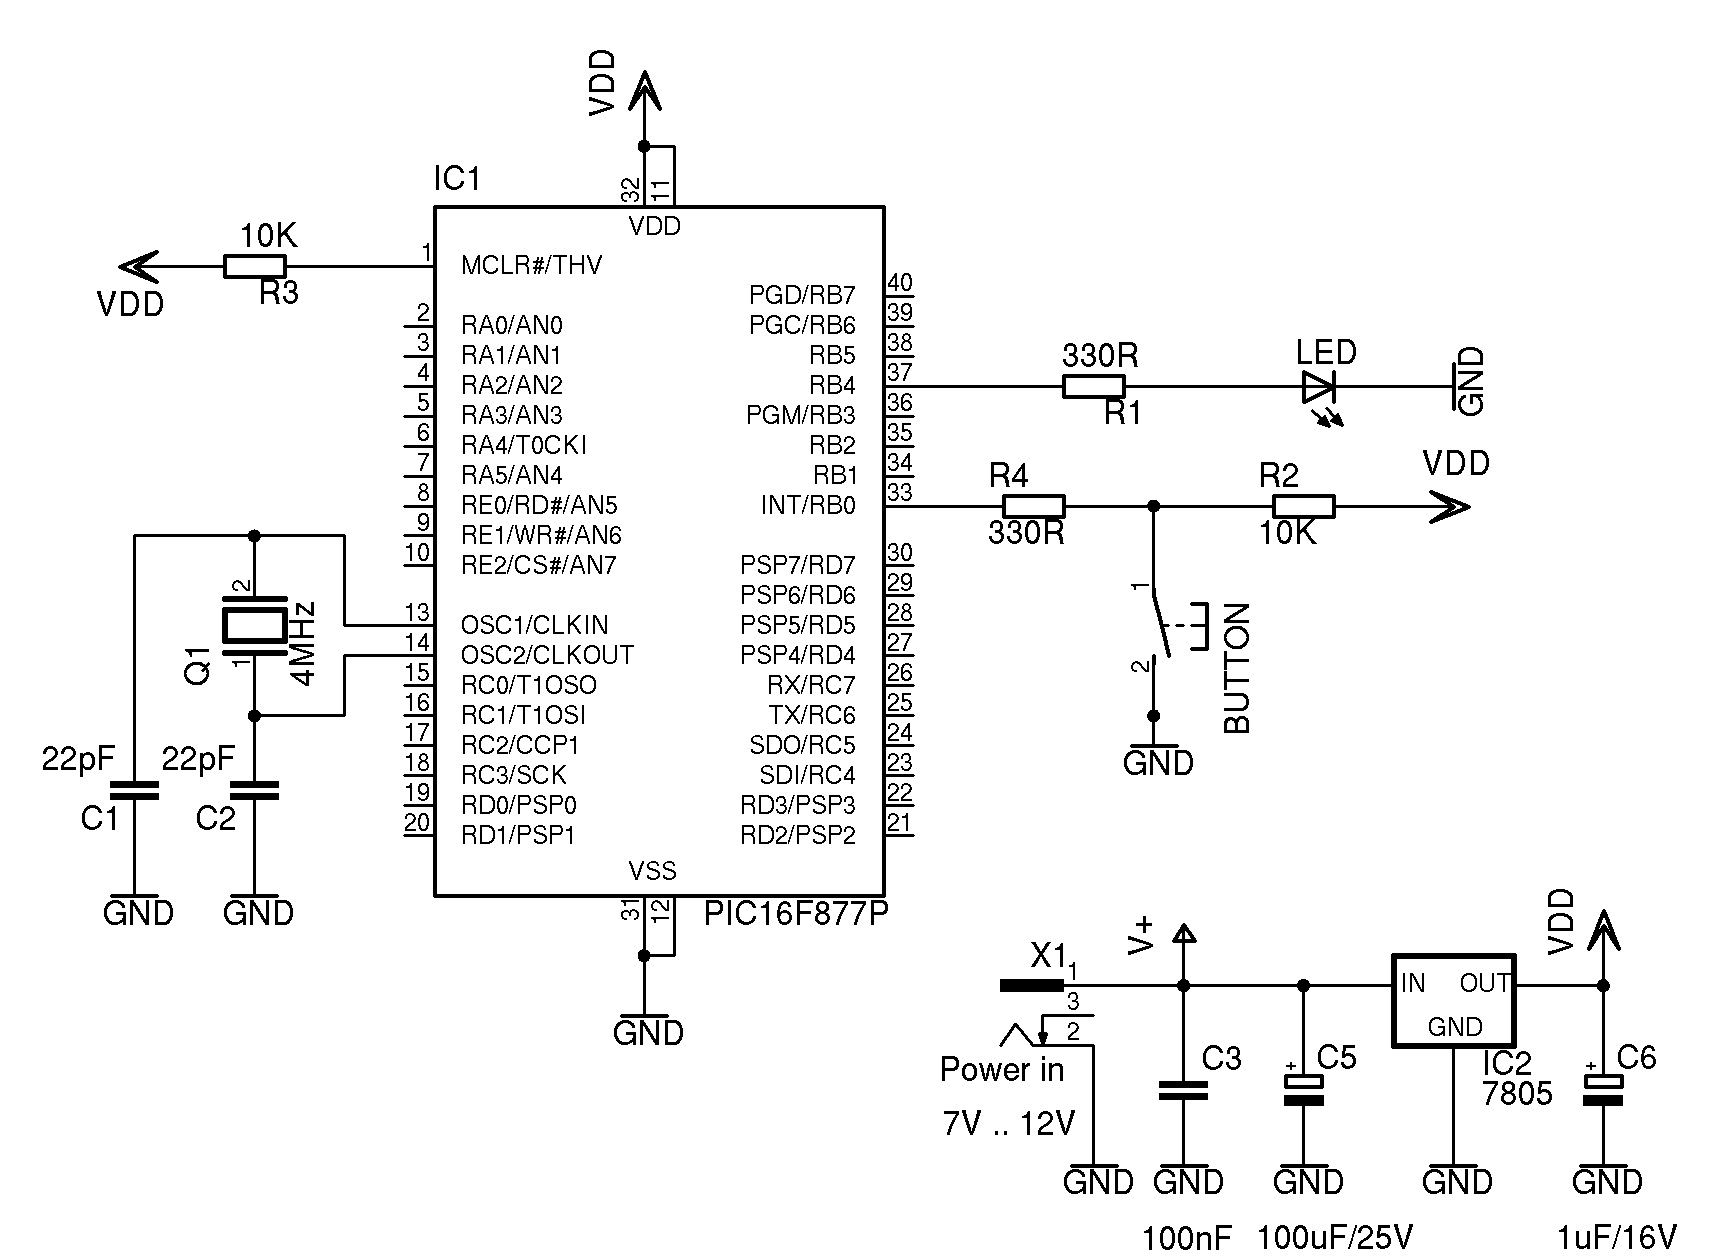
\includegraphics[%
  clip,
  width=15cm,
  keepaspectratio]{esquema.png}

A 47nF to 100nF capacitor is recommended between MCLR and ground.
this will avoid unvanted resets when noisy loads or power supplies
are used.

No PCB layout is given, you are free to build your PCB design.

All example in this section have a number starting each line. These
numbers are only here for teaching purposes and should not be in your
project files.


\section{Example 0: Blink a led.}

\label{sec:Example-0:-Blink}

\begin{quotation}
\textbf{Note}: Line numbers are not included in program but used just
for explanations !
\end{quotation}
\begin{verbatim}     1  -- This must be in the first line
     2  include c16f877
     3  
     4  
     5  
     6  
     7  -- config fuses
     8  pragma target protection off
     9  pragma target debug off
    10  pragma target cdp off
    11  pragma target lvp off
    12  pragma target bor off
    13  pragma target powerup on
    14  pragma target watchdog off
    15  pragma target osc xt
    16  
    17  -- Fosc definition
    18  pragma target clock 4_000_000
    19  
    20  -- PORTB and TRISB definitions
    21  var volatile byte PORTB at {0x06,0x106}
    22  var volatile byte TRISB at {0x86,0x186}
    23  
    24  -- B4 pin definition
    25  var volatile bit pin_b4 at PORTB : 4
    26  
    27  -- Led at pin_b4
    28  var volatile bit LED is pin_b4
    29  
    30  -- 1 second wait procedure
    31  procedure wait_1sec is
    32     for 5 loop
    33        for 6_500 loop  
    34           asm nop
    35        end loop
    36     end loop
    37  end procedure
    38  
    39  
    40  -- Reset PORTB
    41  PORTB = 0
    42  
    43  -- PORTB => all bits output
    44  TRISB = 0b_0000_0000
    45  
    46  -- main loop
    47  forever loop
    48     LED = high  -- LED on
    49     wait_1sec
    50     LED = low   -- LED off
    51     wait_1sec
    52  end loop   
\end{verbatim}


\paragraph{Description}

\begin{description}
\item [1--2]The first line must be an \emph{include} to a PIC chip definition
file%
\footnote{See section \ref{sub:PIC-chip-definition}~\vpageref{sub:PIC-chip-definition}%
}.
\item [7--15]These configuration fuses must match your specific programmer,
etc. Handle with care, a bad configuration will give you a non working
PIC.
\item [17--18]Declare the crystal value being used.
\item [20--25]Declare the PIC port to be used. Both PORTx and TRISx are
needed. Those lines may be omited if a \emph{register definition file}
is included.
\item [27--28]Declare an alias, it's easier to remember.
\item [30--37]A procedure to waste some time. These values will give you
a crude approach to one second delay; modify them and see the effect
of the LED flashing rate. Use just one instruction \verb+FOR 64_910 LOOP+
and see the effect.
\item [40--44]Initialize and configure the port. This initialization part
is usually the first lines of the main code.
\item [46--52]Real main code. Here, an endless loop with our magic LED
blinking sequence: LED on, wait, LED off, wait. The wait sequence
is necessary to see the LED blinking.
\end{description}

\section{Example 1: Scan a button.}

\label{sec:Example-1:-Scan}

\begin{quotation}
\textbf{Note}: Line numbers are not included in program but used just
for explanations !
\end{quotation}
\begin{verbatim}     1  -- This must be in the first line
     2  include c16f877
     3  
     4  
     5  
     6  
     7  -- config fuses
     8  pragma target protection off
     9  pragma target debug off
    10  pragma target cdp off
    11  pragma target lvp off
    12  pragma target bor off
    13  pragma target powerup on
    14  pragma target watchdog off
    15  pragma target osc xt
    16  
    17  -- Fosc definition
    18  pragma target clock 4_000_000
    19  
    20  -- PORTB and TRISB definitions
    21  var volatile byte PORTB at {0x06,0x106}
    22  var volatile byte TRISB at {0x86,0x186}
    23  
    24  -- B0 pin definition
    25  var volatile bit pin_b0 at PORTB : 0
    26  
    27  -- B4 pin definition
    28  var volatile bit pin_b4 at PORTB : 4
    29  
    30  
    31  -- Button at pin_b0
    32  var volatile bit Button is pin_b0
    33  
    34  -- Led at pin_b4
    35  var volatile bit LED is pin_b4
    36  
    37  
    38  -- Reset PORTB
    39  PORTB = 0b_0000_0000
    40  
    41  -- PORTB => b7 ..b1 = output, b0 = input
    42  TRISB = 0b_0000_0001
    43  PORTB = 0b_0000_0001
    44  
    45  -- main loop
    46  forever loop
           -- pressed button pulls pin low, see schematic
    47     if ! Button then   ; Check if Button pressed
    48        LED = on
    49     else               ; ... if not pressed
    50        LED = off
    51     end if
    52  end loop   
\end{verbatim}


\paragraph{Description}

\begin{description}
\item [1--22]See \emph{Example 0} in section \ref{sec:Example-0:-Blink}~1\vpageref{sec:Example-0:-Blink}.
\item [24--35]Add declarations of both elements being used: the LED and
the Button.
\item [38--43]While initializing the port, take care to declare LED pin
as \emph{output} and Button pin as \emph{input}.
\item [47]By pressing the Button, the pin will be tied to Ground%
\footnote{See the circuit in section \ref{sec:Examples}~\vpageref{sec:Examples}.%
}. In order to detect it with the IF statement we must apply a logical
invert to the bit variable. In this way -- on pressing button -- the
logical expression \verb+IF ! Button THEN ...+ of the IF statement
will be true. Button contact bouncing is not prevented in this program.
\item [47--51]LED will be ON when Button is pressed, and will be OFF when
Button is not pressed.
\end{description}

\section{Example 2: Control the blink of a led.}

\label{sec:Example-2:-Control}

\begin{quotation}
\textbf{Note}: Line numbers are not included in program but used just
for explanations !
\end{quotation}
\begin{verbatim} 
     1  -- This must be in the first line
     2  include c16f877
     3  
     4  
     5  
     6  
     7  -- config fuses
     8  pragma target protection off
     9  pragma target debug off
    10  pragma target cdp off
    11  pragma target lvp off
    12  pragma target bor off
    13  pragma target powerup on
    14  pragma target watchdog off
    15  pragma target osc xt
    16  
    17  -- Fosc definition
    18  pragma target clock 4_000_000
    19  
    20  
    21  -- PORTB and TRISB definitions
    22  var volatile byte PORTB at {0x06,0x106}
    23  var volatile byte TRISB at {0x86,0x186}
    24  
    25  -- B0 pin definition
    26  var volatile bit pin_b0 at PORTB : 0
    27  
    28  -- B4 pin definition
    29  var volatile bit pin_b4 at PORTB : 4
    30  
    31  
    32  -- Button at pin_b0
    33  var volatile bit Button is pin_b0
    34  
    35  -- Led at pin_b4
    36  var volatile bit LED is pin_b4
    37  
    38  -- 1 second wait procedure
    39  procedure wait_1sec is
    40     for 5 loop
    41        for 6_500 loop  
    42           asm nop
    43        end loop
    44     end loop
    45  end procedure
    46  
    47  procedure delay_miliseconds is
    48     for 1000 loop
    49        asm nop
    50     end loop
    51  end procedure
    52  
    53  -- Reset PORTB
    54  PORTB = 0b_0000_0000
    55  
    56  -- PORTB => output
    57  TRISB = 0b_0000_0001
    58  PORTB = 0b_0000_0001
    59  
    60  -- main loop
    61  forever loop
    62     if ! Button then   ; Check if Button pressed
    63        delay_milisecons
    64        if ! Button then
    65           ; Check again if Button pressed  
    66           LED = on
    67           wait_1sec
    68           LED = off
    69           wait_1sec
    70         end if
    71     end if
    72  end loop   
\end{verbatim}


\paragraph{Description}

\begin{description}
\item [1--36]See \emph{Example 1} in section \ref{sec:Example-1:-Scan}~1\vpageref{sec:Example-1:-Scan}.
\item [38--45]See \emph{Example 0} in section \ref{sec:Example-0:-Blink}~\vpageref{sec:Example-0:-Blink}.
\item [53--58]See \emph{Example 1} in section \ref{sec:Example-1:-Scan}~1\vpageref{sec:Example-1:-Scan}.
\item [62]See \emph{Example 1} in section \ref{sec:Example-1:-Scan}~1\vpageref{sec:Example-1:-Scan}.
\item [62--71]In this example the LED will blink \emph{only} when Button
is pressed longer than a few miliseconds.
\end{description}

\section{Example 3: Adding a hardware timer.}

\label{sec:Example-3:-TMR0}

\begin{quotation}
\textbf{Note}: Line numbers are not included in program but used just
for explanations !
\end{quotation}
\begin{verbatim}     1  -- This must be in first line
     2  include c16f877
     3  
     4  
     5  
     6  
     7  -- config fuses
     8  pragma target protection off
     9  pragma target debug off
    10  pragma target cdp off
    11  pragma target lvp off
    12  pragma target bor off
    13  pragma target powerup on
    14  pragma target watchdog off
    15  pragma target osc xt
    16  
    17  -- Fosc definition
    18  pragma target clock 4_000_000
    19  
    20  
    21  -- PORTB and TRISB definitions
    22  var volatile byte PORTB at {0x06,0x106}
    23  var volatile byte TRISB at {0x86,0x186}
    24  
    25  -- B0 pin definition
    26  var volatile bit pin_b0 at PORTB : 0
    27  
    28  -- B4 pin definition
    29  var volatile bit pin_b4 at PORTB : 4
    30  
    31  
    32  -- Button at pin_b0
    33  var volatile bit Button is pin_b0
    34  
    35  -- Led at pin_b4
    36  var volatile bit LED is pin_b4
    37  
    38  
    39  -- 1 millisecond wait procedure
    40  -- TMR0_delay=(256-InitTMR0)*4*prescaler/Fosc
    41  -- TMR0_delay=(256-6)*4*4/4_000_000= 1 msec.
    42  --
    43  -- InitTMR0 = 6
    44  -- Prescaler = 1:4
    45  -- Fosc = 4_000_000
    46  --
    47  -- Delay = 0.001 secs
    48  
    49  
    50  -- Init TMR0, free run mode, int osc, prescaler 1:4
    51  var volatile byte TMR0 at {0x01,0x101}
    52  var volatile byte OPTION_REG at {0x81,0x181}
    53  OPTION_REG = 0b_1000_0001
    54  
    55  -- Disable interrupts, reset TMR0 flag
    56  var volatile byte INTCON at {0x0B,0x8B,0x10B,0x18B}
    57  var volatile bit T0if at INTCON : 2
    58  INTCON = 0
    59  
    60  const byte InitTMR0 = 6
    61  
    62  procedure wait_1sec is
    63     for 1_000 loop  
    64        -- Wait for TMR0 1 msec.
    65        while ( ! T0if ) loop
    66        end loop
    67        -- Reset TMR0IF
    68        T0if = low
    69        -- Add InitTMR0
    70        TMR0 = TMR0 + InitTMR0
    71     end loop
    72  end procedure
    73  
    74  
    75  -- Reset PORTB
    76  PORTB = 0b_0000_0000
    77  
    78  -- PORTB => B0 input, B1..B7 output
    79  TRISB = 0b_0000_0001
    80  PORTB = 0b_0000_0001
    81  
    82  
    83  -- main loop
    84  forever loop 
    85     if ! Button then ; Check if Button is 
    86                      ; permanently pressed
    87        LED = on
    88        wait_1sec
    89        LED = off
    90        wait_1sec
    91     end if
    92  end loop   
\end{verbatim}


\paragraph{Description}

\begin{description}
\item [1--36]See \emph{Example 1} in section \ref{sec:Example-1:-Scan}~1\vpageref{sec:Example-1:-Scan}.
\item [39--47]Inline comments with a brief description how to set TMR0.
Take your PIC chip datasheets and read the section entitled \emph{TIMER
0}. The goal in this example is to get a TMR0 overflow each millisecond.
Using a 4MHz crystal, it's necessary a prescaler of 1:4 and init TMR0
with a constant value each time it overflows.
\item [50--58]Declare and initialize the SFRs related with TMR0. See your
PIC chip datasheets, here TMR0 will work in \emph{free running mode}.
\item [62--72]At this point TMR0 overflows each millisecond and will set
a bit called T0IF. The WHILE statement will stop program until T0IF
is set (TMR0 overflow), so we \emph{must} reset this bit and load
TMR0 with the init constant value. Doing these steps 1000 times will
give us one second delay.
\item [75--80]See \emph{Example 1} in section \ref{sec:Example-1:-Scan}~1\vpageref{sec:Example-1:-Scan}.
\item [83--92]In this example the LED will blink \emph{only} when Button
is kept pressed.
\end{description}

\section{Example 4: Using hardware interrupts.}

\label{sec:Example-4:-Interrupts}

\begin{quotation}
\textbf{Note}: Line numbers are not included in program but used just
for explanations !
\end{quotation}
\begin{verbatim}     1  -- This must be in the first line
     2  include c16f877
     3  
     4  
     5  
     6  
     7  -- config fuses
     8  pragma target protection off
     9  pragma target debug off
    10  pragma target cdp off
    11  pragma target lvp off
    12  pragma target bor off
    13  pragma target powerup on
    14  pragma target watchdog off
    15  pragma target osc xt
    16  
    17  -- Fosc definition
    18  pragma target clock 4_000_000
    19  
    20  -- PORTB and TRISB definitions
    21  var volatile byte PORTB at {0x06,0x106}
    22  var volatile byte TRISB at {0x86,0x186}
    23  
    24  -- B0 pin definition
    25  var volatile bit pin_b0 at PORTB : 0
    26  
    27  -- B4 pin definition
    28  var volatile bit pin_b4 at PORTB : 4
    29  
    30  
    31  -- Button at pin_b0
    32  var volatile bit Button is pin_b0
    33  
    34  -- Led at pin_b4
    35  var volatile bit LED is pin_b4
    36  
    37  
    38  -- 1 millisecond delay
    39  -- TMR0_delay=(256-InitTMR0)*4*prescaler/Fosc
    40  -- TMR0_delay=(256-6)*4*4/4_000_000= 1 msec.
    41  --
    42  -- InitTMR0 = 6
    43  -- Prescaler = 1:4
    44  -- Fosc = 4_000_000
    45  --
    46  -- Delay = 0.001 secs
    47  
    48  -- RB0INT falling edge, Init TMR0, free run mode,
    49  -- int osc, prescaler 1:4
    50  var volatile byte TMR0 at {0x01,0x101}
    51  var volatile byte OPTION_REG at {0x81,0x181}
    52  OPTION_REG = 0b_1000_0001
    53  
    54  -- Enable TMR0 interrupt, RB0INT interrupt, reset flags
    55  var volatile byte INTCON at {0x0B,0x8B,0x10B,0x18B}
    56  var volatile bit T0if at INTCON : 2
    57  var volatile bit INTf at INTCON : 1
    58  var volatile bit INTE at INTCON : 4
    59  var volatile bit T0IE at INTCON : 5
    60  INTCON = 0B_1011_0000
    61  const byte InitTMR0 = 6
    62  var volatile bit Enable_Button is INTE
    63  var volatile bit Enable_Timmer is T0IE
    64  
    65  Enable_Timmer = off
    66  Enable_Button = on
    67  
    68  -- declare vars
    69  var word milisec_count
    70  var bit Flag_tmr0 = false, Flag_rb0int = false
    71  
    72  -- TMR0 interrupt
    73  procedure TMR0_ISR is
    74  pragma interrupt
    75     if T0if then
    76        -- Reset TMR0IF
    77        T0if = low
    78        -- Reset InitTMR0
    79        TMR0 = InitTMR0
    80        -- add one count
    81        milisec_count = milisec_count + 1
    82        -- Check count 1_000
    83        if milisec_count == 1_000 then
    84           -- if 1000 msecs. => Activate flag
    85           Flag_tmr0 = true
    86           -- reset counter
    87           milisec_count = 0 
    88        end if
    89     end if
    90  end procedure
    91  
    92  -- RB0INT interrupt
    93  procedure RB0INT_ISR is
    94  pragma interrupt
    95     if INTf then
    96        -- Reset TMR0IF
    97        INTf = low
    98        -- Activate flag
    99        Flag_rb0int = true
   100        -- reset counter
   101        milisec_count = 0
   102        TMR0 = 6
   103        -- Enable timmer
   104        Enable_Timmer = on
   105     end if
   106  end procedure
   107  
   108  
   109  -- Reset PORTB
   110  PORTB = 0b_0000_0000
   111  
   112  -- PORTB => B0 input, B1..B7 output
   113  TRISB = 0b_0000_0001
   114  PORTB = 0b_0000_0001
   115  
   116  
   117  -- main loop
   118  forever loop
   119     if Flag_rb0int then   ; Check if Button pressed
   120        -- Disable Button interrupt
   121        Enable_Button = low
   122        -- Turn on LED
   123        LED = on
   124        -- Wait for 1 sec event
   125        while ( ! Flag_tmr0 ) loop
   126        end loop
   127        -- Clear flag
   128        Flag_tmr0 = low
   129        -- Turn off LED
   130        LED = off
   131        -- Wait for 1 sec event
   132        while ( ! Flag_tmr0 ) loop
   133        end loop
   134        -- Clear flag
   135        Flag_tmr0 = low
   136        -- Enable Button interrupt
   137        Enable_Button = High
   138        -- Disable timmer interrupt
   139        Enable_Timmer = low
   140        -- Clear flags
   141        Flag_rb0int = low
   142        Flag_tmr0 = low
   143     end if
   144  end loop   
\end{verbatim}


\paragraph{Description}

\begin{description}
\item [1--35]See \emph{Example 1} in section \ref{sec:Example-1:-Scan}~1\vpageref{sec:Example-1:-Scan}.
\item [38--46]See \emph{Example 3} in section \ref{sec:Example-3:-TMR0}~1\vpageref{sec:Example-3:-TMR0}.
\item [49--52]Declare and initialize the SFRs related with TMR0. See your
PIC chip datasheets, here TMR0 will work in \emph{free running mode}.
Set also RB0INT edge detection to \emph{falling edge}.
\item [54--60]Declare and configure TMR0 and RB0INT interrupts
\item [62--66]Declare some alias, it's easier to remember.
\item [68--70]Declare some variables to be used globally. \verb+Flag_tmr0+
and \verb+Flag_rb0in+ will be used by main program to know about
interrupt events.
\item [72--90]TMR0 interrupt procedure.
\item [75]Check if is exactly TMR0 interrupt.
\item [76--79]Reset flag and init TMR0 again.
\item [80--81]Add one count to our \emph{1000 milliseconds} count.
\item [82--88]On reaching the 1000 milliseconds count, set \verb+Flag_tmr0+
and reset internal count.
\item [92--106]RB0INT interrupt procedure.
\item [95]Check if is exactly RB0INT interrupt.
\item [96--97]Reset flag RB0INT.
\item [98--105]Set \verb+Flag_rb0in+, enable TMR0 (will be disabled anywhere)
and reset TMR0 count. In this way TMR0 will start counting only when
Button is pressed.
\item [109--114]See \emph{Example 1} in section \ref{sec:Example-1:-Scan}~\vpageref{sec:Example-1:-Scan}.
\item [117-144]Main code. In this example the LED will blink only once
each time Button is pressed. 
\item [119]Scan Button testing \verb+Flag_rb0in+ bit. The interrupt procedure
will do all hard job.
\item [120--123]Disable future Button interrupt events.
\item [122--135]The \emph{magic sequence} to blink a LED.
\item [124--128]Turn on LED and wait for one second by testing \verb+Flag_tmr0+.
Clear flag for next use.
\item [129--135]Turn off LED and wait for one second by testing \verb+Flag_tmr0+.
Clear flag for next use.
\item [136--142]Enable Button interrupt events again, disable TMR0 interrupt
events (work already done in this loop) and clear both flags. 
\end{description}

\chapter{Glossary}

\begin{description}
\item [ACCESSOR]An accessor method is a method that is usually small, simple
and provides the means for the state of an object to be accessed from
other parts of a program. An accessor method that changes the state
of an object is often called an update method or, sometimes, mutator
method. Objects that provide such methods are considered mutable objects.
See Wikipedia~\cite{Wikipedia}, keyword: Accessor.
\end{description}
\html{\\}

\begin{description}
\item [ANALOG~DEVICE]An analog device is a component of a electronic circuit
that change its properties continuously in both time and amplitude.
It differs from digital devices in that small fluctuations in the
signal are meaningful in that they are continuously variable rather
than digitally quantised.
\end{description}
\html{\\}

\begin{description}
\item [ATOMIC]A single operation, with single as in \emph{non interuptable}.
It has to finish before anything else can be done. Which implies that
a \emph{singe operation} might take more than one machine instruction
but they all must finisch before any interupt can interfere with the
processor. On most processors \emph{atomic} is equivalent to one \emph{instruction}.
\end{description}
\html{\\}

\begin{description}
\item [BANK]see MEMORY BANK.
\end{description}
\html{\\}

\begin{description}
\item [BINARY~CONSTANT]Begins with \verb+"0b"+ and continues until the
first character not in the set \{\verb+"_"+, \verb+"0"+, \verb+"1"+\}.
It's fully evaluated at compile time.
\end{description}
\html{\\}

\begin{description}
\item [BIT]or \emph{binary digit.} Is the smallest unit of data and has
a boolean value.
\end{description}
\html{\\}

\begin{description}
\item [BITMASK]also MASK. Extracts the status of certain bits in a binary
string or number.
\end{description}
\html{\\}

\begin{description}
\item [BITWISE~OPERATOR]Operates on individual BITs of one or two operands.
See Wikipedia~\cite{Wikipedia}, keyword: Bitwise.
\end{description}
\html{\\}

\begin{description}
\item [BITWISE~COMPLEMENT]An operator that changes all BITs of an operand
from 1 to 0 or vice versa. See Wikipedia~\cite{Wikipedia}, keyword:
One's\_complement.
\end{description}
\html{\\}

\begin{description}
\item [BITWISE~AND]An operator that takes two bit patterns of equal length,
and produces another one of the same length by matching up corresponding
bits (the first of each; the second of each; and so on) and performing
the logical AND operation on each pair of corresponding bits. In each
pair, the result is 1 if the first bit is 1 AND the second bit is
1. Otherwise, the result is zero. See Wikipedia~\cite{Wikipedia},
keyword: Bitwise.
\end{description}
\html{\\}

\begin{description}
\item [BITWISE~OR]An operator that takes two bit patterns of equal length,
and produces another one of the same length by matching up corresponding
bits (the first of each; the second of each; and so on) and performing
the logical OR operation on each pair of corresponding bits. In each
pair, the result is 1 if the first bit is 1 OR the second bit is 1.
Otherwise, the result is zero. See Wikipedia~\cite{Wikipedia}, keyword:
Bitwise.
\end{description}
\html{\\}

\begin{description}
\item [BITWISE~XOR]An operator that takes two bit patterns of equal length,
and produces another one of the same length by matching up corresponding
bits (the first of each; the second of each; and so on) and performing
the logical OR operation on each pair of corresponding bits. In each
pair, the result is 1 if the two bits are different, and 0 if they
are the same. See Wikipedia~\cite{Wikipedia}, keyword: Bitwise.
\end{description}
\html{\\}

\begin{description}
\item [BOOLEAN]Boolean logic is a form of algebra in which all values are
reduced to either TRUE or FALSE. In \pjal\ this means TRUE or FALSE,
also ON or OFF are valid and either 1 and 0. See Wikipedia~\cite{Wikipedia},
keyword: Boolean.
\end{description}
\html{\\}

\begin{description}
\item [CONTACT~BOUNCE]Contact bounce is a common problem with mechanical
switches and relays. When the contacts strike together, their momentum
and elasticity act together to cause bounce. The result is a rapidly
pulsed electrical current instead of a clean transition from zero
to full current. If the switch voltage is fed directly to the input
of a microprocessor, then the software might become confused by the
rapid sequence of high and low logic levels when it is expecting only
a single, stable transition between \char`\"{}on\char`\"{} and \char`\"{}off\char`\"{}.
See Wikipedia~\cite{Wikipedia}, keyword: Switch.
\end{description}
\html{\\}

\begin{description}
\item [COMPILER~DIRECTIVE]Data embedded in source code to tell the compiler
some intention about compilation. See Wikipedia~\cite{Wikipedia},
keyword: Compiler\_directive.
\end{description}
\html{\\}

\begin{description}
\item [CO-OPERATIVE~MULTITASKING](or non-preemptive multitasking) is a
form of multitasking in which multiple tasks execute by voluntarily
ceding control to other tasks at programmer-defined points within
each task. See Wikipedia~\cite{Wikipedia}, keyword: Co-operative\_multitasking.
\end{description}
\html{\\}

\begin{description}
\item [DECIMAL~CONSTANT]Begins with a digit, and continues until the first
character not in the set \{\verb+"_"+, digit\}. It's fully evaluated
at compile time.
\end{description}
\html{\\}

\begin{description}
\item [DECLARATION]Specifies a variable's dimensions, identifier, type,
and other aspects.
\end{description}
\html{\\}

\begin{description}
\item [DIGIT]A character in the set \{\verb+"0"+--\verb+"9"+\}.
\end{description}
\html{\\}

\begin{description}
\item [ENDIANNESS]The two main types of endianness are known as big-endian
and little-endian. In \emph{big-endian}, the most significant byte
(MSB) is stored at the memory location with the lowest address. In
\emph{little-endian}, the least significant byte (LSB) is stored at
the memory location with the lowest address. pJAL and PICs uses \emph{little-endian}
memory management. See Wikipedia~\cite{Wikipedia}, keyword: Endianness.
\end{description}
\html{\\}

\begin{description}
\item [EXPRESSION]Anything that evaluates to a value, for example x + 1.
\end{description}
\html{\\}

\begin{description}
\item [IDENTIFIER]Begins with a member of the set \{\verb+"_"+, \verb+"a"+--\verb+"z"+,
\verb+"A"+--\verb+"Z"+\} and continues until the first character
\emph{NOT} in the set \{\verb+"_"+, \verb+"a"+--\verb+"z"+, \verb+"A"+--\verb+"Z"+,
digit\}.
\end{description}
\html{\\}

\begin{description}
\item [INTERRUPT]is an asynchronous signal from hardware (or software)
indicating the need for attention. Originated as a way to avoid wasting
the processors valuable time in polling loops, waiting for external
events. Instead, an interrupt signals the processor when an event
occurs, allowing the processor to process other work while the event
is pending. See Wikipedia~\cite{Wikipedia}, keyword: Interrupt.
\end{description}
\html{\\}

\begin{description}
\item [HEXADECIMAL~CONSTANT]Begins with \verb+"0x"+ and continues until
the first character not in the set \{\verb+"_"+, \verb+"0"+--\verb+"9"+,
\verb+"a"+--\verb+"f"+, \verb+"A"+--\verb+"F"+\}. It's fully evaluated
at compile time.
\end{description}
\html{\\}

\begin{description}
\item [LOGICAL~EXPRESSION]The result is 0 if the expression evaluation
is zero, and 1 if the expression evaluation is anything other than
0.
\end{description}
\html{\\}

\begin{description}
\item [LOGICAL~NOT]An operator that changes the boolean state from TRUE
to FALSE or vice versa. 
\end{description}
\html{\\}

\begin{description}
\item [LSB]It is the byte in that position of a multi-byte number which
has the least potential value. If it's written in lowercase, means
the lowest BIT. See Wikipedia~\cite{Wikipedia}, keyword: Least\_significant\_byte.
\end{description}
\html{\\}

\begin{description}
\item [MEMORY~BANK]PIC architecture typically has more memory registers
than can be addressed in a single byte address. A special SFR register
is utilized to switch to another bank of memory where the base addresses
repeat. Check the specific PIC datasheet to determine the number of
banks and their size. 
\end{description}
\html{\\}

\begin{description}
\item [MODULO]The modulo operation finds the remainder of division.
\end{description}
\html{\\}

\begin{description}
\item [MSB]It is the byte in that position of a multi-byte number which
has the greatest potential value. If it's written in lowercase, means
the greatest BIT. See Wikipedia~\cite{Wikipedia}, keyword: Most\_significant\_byte.
\end{description}
\html{\\}

\begin{description}
\item [MULTITASKING]is a method by which multiple tasks, also known as
processes, share common processing resources such as a CPU. See Wikipedia~\cite{Wikipedia},
keyword: Computer\_multitasking.
\end{description}
\html{\\}

\begin{description}
\item [NIBBLE]Half of a an 8 bit byte, a group of 4 bits. Corresponding
\pjal\ \emph{type} is BIT{*}4, eg: you can send data to a HD44780
LCD in nibble (4 bit) mode. 
\end{description}
\html{\\}

\begin{description}
\item [OCTAL~CONSTANT]Begins with \verb+"0q"+ and continues until the
first character not in the set \{\verb+"_"+, \verb+"0"+--\verb+"7"+\}.
It's fully evaluated at compile time.
\end{description}
\html{\\}

\begin{description}
\item [OPERATOR]The most basic mathematical or logical functions usually
represented by a single character eg: + - {*} 
\end{description}
\html{\\}

\begin{description}
\item [OPERAND]One of the inputs (arguments) of an operator. 
\end{description}
\html{\\}

\begin{description}
\item [PRAGMA](short for \char`\"{}\emph{pragmatic information}\char`\"{}),
see COMPILER DIRECTIVE.
\end{description}
\html{\\}

\begin{description}
\item [STRING~CONSTANT]Begins with \verb+'+ and continues until the next
\verb+'+. Also, begins with \verb+"+ and continues until the next
\verb+"+. It's fully evaluated at compile time.
\end{description}
\html{\\}

\begin{description}
\item [TOKENS]\pjal\ syntax is based on tokens. In programming languages,
a single element of a programming language. In \pjal\ can be an identifier,
constant, operator, or any non-space character. See Wikipedia~\cite{Wikipedia},
keyword: Token.
\end{description}
\html{\\}

\begin{description}
\item [TRINARY~OPERATOR]An operator which three operands are associated
with the operator. Example: in C programming language the \verb+?+
operator, \verb+c?a:b+.
\end{description}
\html{\\}

\begin{description}
\item [UNARY~OPERATOR]Also MONADIC operator. An operator which only takes
one operand (argument), eg: -1 (a negative value).
\end{description}
\html{\\}

\begin{description}
\item [VAR]Variable.
\end{description}
\html{\\}


\chapter{GNU Free Documentation License}

\label{sec:GNU-FDL}

GNU Free Documentation License

Version 1.2, November 2002

Copyright (C) 2000,2001,2002 Free Software Foundation, Inc.

51 Franklin St, Fifth Floor, Boston, MA 02110-1301 USA

Everyone is permitted to copy and distribute verbatim copies of this
license document, but changing it is not allowed.

0. PREAMBLE

The purpose of this License is to make a manual, textbook, or other
functional and useful document \char`\"{}free\char`\"{} in the sense
of freedom: to assure everyone the effective freedom to copy and redistribute
it, with or without modifying it, either commercially or noncommercially.
Secondarily, this License preserves for the author and publisher a
way to get credit for their work, while not being considered responsible
for modifications made by others.

This License is a kind of \char`\"{}copyleft\char`\"{}, which means
that derivative works of the document must themselves be free in the
same sense. It complements the GNU General Public License, which is
a copyleft license designed for free software.

We have designed this License in order to use it for manuals for free
software, because free software needs free documentation: a free program
should come with manuals providing the same freedoms that the software
does. But this License is not limited to software manuals; it can
be used for any textual work, regardless of subject matter or whether
it is published as a printed book. We recommend this License principally
for works whose purpose is instruction or reference.

1. APPLICABILITY AND DEFINITIONS

This License applies to any manual or other work, in any medium, that
contains a notice placed by the copyright holder saying it can be
distributed under the terms of this License. Such a notice grants
a world-wide, royalty-free license, unlimited in duration, to use
that work under the conditions stated herein. The \char`\"{}Document\char`\"{},
below, refers to any such manual or work. Any member of the public
is a licensee, and is addressed as \char`\"{}you\char`\"{}. You accept
the license if you copy, modify or distribute the work in a way requiring
permission under copyright law.

A \char`\"{}Modified Version\char`\"{} of the Document means any work
containing the Document or a portion of it, either copied verbatim,
or with modifications and/or translated into another language.

A \char`\"{}Secondary Section\char`\"{} is a named appendix or a front-matter
section of the Document that deals exclusively with the relationship
of the publishers or authors of the Document to the Document's overall
subject (or to related matters) and contains nothing that could fall
directly within that overall subject. (Thus, if the Document is in
part a textbook of mathematics, a Secondary Section may not explain
any mathematics.) The relationship could be a matter of historical
connection with the subject or with related matters, or of legal,
commercial, philosophical, ethical or political position regarding
them.

The \char`\"{}Invariant Sections\char`\"{} are certain Secondary Sections
whose titles are designated, as being those of Invariant Sections,
in the notice that says that the Document is released under this License.
If a section does not fit the above definition of Secondary then it
is not allowed to be designated as Invariant. The Document may contain
zero Invariant Sections. If the Document does not identify any Invariant
Sections then there are none.

The \char`\"{}Cover Texts\char`\"{} are certain short passages of
text that are listed, as Front-Cover Texts or Back-Cover Texts, in
the notice that says that the Document is released under this License.
A Front-Cover Text may be at most 5 words, and a Back-Cover Text may
be at most 25 words.

A \char`\"{}Transparent\char`\"{} copy of the Document means a machine-readable
copy, represented in a format whose specification is available to
the general public, that is suitable for revising the document straightforwardly
with generic text editors or (for images composed of pixels) generic
paint programs or (for drawings) some widely available drawing editor,
and that is suitable for input to text formatters or for automatic
translation to a variety of formats suitable for input to text formatters.
A copy made in an otherwise Transparent file format whose markup,
or absence of markup, has been arranged to thwart or discourage subsequent
modification by readers is not Transparent. An image format is not
Transparent if used for any substantial amount of text. A copy that
is not \char`\"{}Transparent\char`\"{} is called \char`\"{}Opaque\char`\"{}.

Examples of suitable formats for Transparent copies include plain
ASCII without markup, Texinfo input format, \LaTeX{} input format,
SGML or XML using a publicly available DTD, and standard-conforming
simple HTML, PostScript or PDF designed for human modification. Examples
of transparent image formats include PNG, XCF and JPG. Opaque formats
include proprietary formats that can be read and edited only by proprietary
word processors, SGML or XML for which the DTD and/or processing tools
are not generally available, and the machine-generated HTML, PostScript
or PDF produced by some word processors for output purposes only.

The \char`\"{}Title Page\char`\"{} means, for a printed book, the
title page itself, plus such following pages as are needed to hold,
legibly, the material this License requires to appear in the title
page. For works in formats which do not have any title page as such,
\char`\"{}Title Page\char`\"{} means the text near the most prominent
appearance of the work's title, preceding the beginning of the body
of the text.

A section \char`\"{}Entitled XYZ\char`\"{} means a named subunit of
the Document whose title either is precisely XYZ or contains XYZ in
parentheses following text that translates XYZ in another language.
(Here XYZ stands for a specific section name mentioned below, such
as \char`\"{}Acknowledgements\char`\"{}, \char`\"{}Dedications\char`\"{},
\char`\"{}Endorsements\char`\"{}, or \char`\"{}History\char`\"{}.)
To \char`\"{}Preserve the Title\char`\"{} of such a section when you
modify the Document means that it remains a section \char`\"{}Entitled
XYZ\char`\"{} according to this definition.

The Document may include Warranty Disclaimers next to the notice which
states that this License applies to the Document. These Warranty Disclaimers
are considered to be included by reference in this License, but only
as regards disclaiming warranties: any other implication that these
Warranty Disclaimers may have is void and has no effect on the meaning
of this License.

2. VERBATIM COPYING

You may copy and distribute the Document in any medium, either commercially
or noncommercially, provided that this License, the copyright notices,
and the license notice saying this License applies to the Document
are reproduced in all copies, and that you add no other conditions
whatsoever to those of this License. You may not use technical measures
to obstruct or control the reading or further copying of the copies
you make or distribute. However, you may accept compensation in exchange
for copies. If you distribute a large enough number of copies you
must also follow the conditions in section 3.

You may also lend copies, under the same conditions stated above,
and you may publicly display copies.

3. COPYING IN QUANTITY

If you publish printed copies (or copies in media that commonly have
printed covers) of the Document, numbering more than 100, and the
Document's license notice requires Cover Texts, you must enclose the
copies in covers that carry, clearly and legibly, all these Cover
Texts: Front-Cover Texts on the front cover, and Back-Cover Texts
on the back cover. Both covers must also clearly and legibly identify
you as the publisher of these copies. The front cover must present
the full title with all words of the title equally prominent and visible.
You may add other material on the covers in addition. Copying with
changes limited to the covers, as long as they preserve the title
of the Document and satisfy these conditions, can be treated as verbatim
copying in other respects.

If the required texts for either cover are too voluminous to fit legibly,
you should put the first ones listed (as many as fit reasonably) on
the actual cover, and continue the rest onto adjacent pages.

If you publish or distribute Opaque copies of the Document numbering
more than 100, you must either include a machine-readable Transparent
copy along with each Opaque copy, or state in or with each Opaque
copy a computer-network location from which the general network-using
public has access to download using public-standard network protocols
a complete Transparent copy of the Document, free of added material.
If you use the latter option, you must take reasonably prudent steps,
when you begin distribution of Opaque copies in quantity, to ensure
that this Transparent copy will remain thus accessible at the stated
location until at least one year after the last time you distribute
an Opaque copy (directly or through your agents or retailers) of that
edition to the public.

It is requested, but not required, that you contact the authors of
the Document well before redistributing any large number of copies,
to give them a chance to provide you with an updated version of the
Document.

4. MODIFICATIONS

You may copy and distribute a Modified Version of the Document under
the conditions of sections 2 and 3 above, provided that you release
the Modified Version under precisely this License, with the Modified
Version filling the role of the Document, thus licensing distribution
and modification of the Modified Version to whoever possesses a copy
of it. In addition, you must do these things in the Modified Version:

\begin{labeling}{00.00.0000}
\item [A.]Use in the Title Page (and on the covers, if any) a title distinct
from that of the Document, and from those of previous versions (which
should, if there were any, be listed in the History section of the
Document). You may use the same title as a previous version if the
original publisher of that version gives permission.
\item [B.]List on the Title Page, as authors, one or more persons or entities
responsible for authorship of the modifications in the Modified Version,
together with at least five of the principal authors of the Document
(all of its principal authors, if it has fewer than five), unless
they release you from this requirement.
\item [C.]State on the Title page the name of the publisher of the Modified
Version, as the publisher.
\item [D.]Preserve all the copyright notices of the Document.
\item [E.]Add an appropriate copyright notice for your modifications adjacent
to the other copyright notices.
\item [F.]Include, immediately after the copyright notices, a license notice
giving the public permission to use the Modified Version under the
terms of this License, in the form shown in the Addendum below.
\item [G.]Preserve in that license notice the full lists of Invariant Sections
and required Cover Texts given in the Document's license notice.
\item [H.]Include an unaltered copy of this License.
\item [I.]Preserve the section Entitled \char`\"{}History\char`\"{}, Preserve
its Title, and add to it an item stating at least the title, year,
new authors, and publisher of the Modified Version as given on the
Title Page. If there is no section Entitled \char`\"{}History\char`\"{}
in the Document, create one stating the title, year, authors, and
publisher of the Document as given on its Title Page, then add an
item describing the Modified Version as stated in the previous sentence.
\item [J.]Preserve the network location, if any, given in the Document
for public access to a Transparent copy of the Document, and likewise
the network locations given in the Document for previous versions
it was based on. These may be placed in the \char`\"{}History\char`\"{}
section. You may omit a network location for a work that was published
at least four years before the Document itself, or if the original
publisher of the version it refers to gives permission.
\item [K.]For any section Entitled \char`\"{}Acknowledgements\char`\"{}
or \char`\"{}Dedications\char`\"{}, Preserve the Title of the section,
and preserve in the section all the substance and tone of each of
the contributor acknowledgements and/or dedications given therein.
\item [L.]Preserve all the Invariant Sections of the Document, unaltered
in their text and in their titles. Section numbers or the equivalent
are not considered part of the section titles.
\item [M.]Delete any section Entitled \char`\"{}Endorsements\char`\"{}.
Such a section may not be included in the Modified Version.
\item [N.]Do not retitle any existing section to be Entitled \char`\"{}Endorsements\char`\"{}
or to conflict in title with any Invariant Section.
\item [O.]Preserve any Warranty Disclaimers.
\end{labeling}
If the Modified Version includes new front-matter sections or appendices
that qualify as Secondary Sections and contain no material copied
from the Document, you may at your option designate some or all of
these sections as invariant. To do this, add their titles to the list
of Invariant Sections in the Modified Version's license notice. These
titles must be distinct from any other section titles.

You may add a section Entitled \char`\"{}Endorsements\char`\"{}, provided
it contains nothing but endorsements of your Modified Version by various
parties--for example, statements of peer review or that the text has
been approved by an organization as the authoritative definition of
a standard.

You may add a passage of up to five words as a Front-Cover Text, and
a passage of up to 25 words as a Back-Cover Text, to the end of the
list of Cover Texts in the Modified Version. Only one passage of Front-Cover
Text and one of Back-Cover Text may be added by (or through arrangements
made by) any one entity. If the Document already includes a cover
text for the same cover, previously added by you or by arrangement
made by the same entity you are acting on behalf of, you may not add
another; but you may replace the old one, on explicit permission from
the previous publisher that added the old one.

The author(s) and publisher(s) of the Document do not by this License
give permission to use their names for publicity for or to assert
or imply endorsement of any Modified Version.

5. COMBINING DOCUMENTS

You may combine the Document with other documents released under this
License, under the terms defined in section 4 above for modified versions,
provided that you include in the combination all of the Invariant
Sections of all of the original documents, unmodified, and list them
all as Invariant Sections of your combined work in its license notice,
and that you preserve all their Warranty Disclaimers.

The combined work need only contain one copy of this License, and
multiple identical Invariant Sections may be replaced with a single
copy. If there are multiple Invariant Sections with the same name
but different contents, make the title of each such section unique
by adding at the end of it, in parentheses, the name of the original
author or publisher of that section if known, or else a unique number.
Make the same adjustment to the section titles in the list of Invariant
Sections in the license notice of the combined work.

In the combination, you must combine any sections Entitled \char`\"{}History\char`\"{}
in the various original documents, forming one section Entitled \char`\"{}History\char`\"{};
likewise combine any sections Entitled \char`\"{}Acknowledgements\char`\"{},
and any sections Entitled \char`\"{}Dedications\char`\"{}. You must
delete all sections Entitled \char`\"{}Endorsements\char`\"{}.

6. COLLECTIONS OF DOCUMENTS

You may make a collection consisting of the Document and other documents
released under this License, and replace the individual copies of
this License in the various documents with a single copy that is included
in the collection, provided that you follow the rules of this License
for verbatim copying of each of the documents in all other respects.

You may extract a single document from such a collection, and distribute
it individually under this License, provided you insert a copy of
this License into the extracted document, and follow this License
in all other respects regarding verbatim copying of that document.

7. AGGREGATION WITH INDEPENDENT WORKS

A compilation of the Document or its derivatives with other separate
and independent documents or works, in or on a volume of a storage
or distribution medium, is called an \char`\"{}aggregate\char`\"{}
if the copyright resulting from the compilation is not used to limit
the legal rights of the compilation's users beyond what the individual
works permit. When the Document is included in an aggregate, this
License does not apply to the other works in the aggregate which are
not themselves derivative works of the Document.

If the Cover Text requirement of section 3 is applicable to these
copies of the Document, then if the Document is less than one half
of the entire aggregate, the Document's Cover Texts may be placed
on covers that bracket the Document within the aggregate, or the electronic
equivalent of covers if the Document is in electronic form. Otherwise
they must appear on printed covers that bracket the whole aggregate.

8. TRANSLATION

Translation is considered a kind of modification, so you may distribute
translations of the Document under the terms of section 4. Replacing
Invariant Sections with translations requires special permission from
their copyright holders, but you may include translations of some
or all Invariant Sections in addition to the original versions of
these Invariant Sections. You may include a translation of this License,
and all the license notices in the Document, and any Warranty Disclaimers,
provided that you also include the original English version of this
License and the original versions of those notices and disclaimers.
In case of a disagreement between the translation and the original
version of this License or a notice or disclaimer, the original version
will prevail.

If a section in the Document is Entitled \char`\"{}Acknowledgements\char`\"{},
\char`\"{}Dedications\char`\"{}, or \char`\"{}History\char`\"{}, the
requirement (section 4) to Preserve its Title (section 1) will typically
require changing the actual title.

9. TERMINATION

You may not copy, modify, sublicense, or distribute the Document except
as expressly provided for under this License. Any other attempt to
copy, modify, sublicense or distribute the Document is void, and will
automatically terminate your rights under this License. However, parties
who have received copies, or rights, from you under this License will
not have their licenses terminated so long as such parties remain
in full compliance.

10. FUTURE REVISIONS OF THIS LICENSE

The Free Software Foundation may publish new, revised versions of
the GNU Free Documentation License from time to time. Such new versions
will be similar in spirit to the present version, but may differ in
detail to address new problems or concerns. 

See http://www.gnu.org/copyleft.

Each version of the License is given a distinguishing version number.
If the Document specifies that a particular numbered version of this
License \char`\"{}or any later version\char`\"{} applies to it, you
have the option of following the terms and conditions either of that
specified version or of any later version that has been published
(not as a draft) by the Free Software Foundation. If the Document
does not specify a version number of this License, you may choose
any version ever published (not as a draft) by the Free Software Foundation.

ADDENDUM: How to use this License for your documents To use this License
in a document you have written, include a copy of the License in the
document and put the following copyright and license notices just
after the title page:

Copyright (c) YEAR YOUR NAME.

Permission is granted to copy, distribute and/or modify this document
under the terms of the GNU Free Documentation License, Version 1.2
or any later version published by the Free Software Foundation; with
no Invariant Sections, no Front-Cover Texts, and no Back-Cover Texts.
A copy of the license is included in the section entitled \char`\"{}GNU
Free Documentation License\char`\"{}.

If you have Invariant Sections, Front-Cover Texts and Back-Cover Texts,
replace the \char`\"{}with ... Texts''. line with this:

with the Invariant Sections being LIST THEIR TITLES, with the Front-Cover
Texts being LIST, and with the Back-Cover Texts being LIST.

If you have Invariant Sections without Cover Texts, or some other
combination of the three, merge those two alternatives to suit the
situation.

If your document contains nontrivial examples of program code, we
recommend releasing these examples in parallel under your choice of
free software license, such as the GNU General Public License, to
permit their use in free software.

\renewcommand{\bibname}{References}

\begin{thebibliography}{1}
\bibitem{Microchip-web}Microchip's homepage: \htmladdnormallink{http://www.microchip.com}{http://www.microchip.com} 
\bibitem{PICbsc}PICbsc's homepage: \htmladdnormallink{http://www.casadeyork.com/robot/picbsc}{http://www.casadeyork.com/robot/picbsc}
\bibitem{pJALdownload}\pjal\ download homepage: \htmladdnormallink{http://www.casadeyork.com/pjal}{http://www.casadeyork.com/pjal}
\bibitem{Wouter-web}\noun{Wouter van Ooijen}'s homesite: \htmladdnormallink{http://www.voti.nl/jal}{http://www.voti.nl/jal}
\bibitem{Wikipedia}Wikipedia's homepage: \htmladdnormallink{http://en.wikipedia.org}{http://en.wikipedia.org}
\bibitem{JAL-SF-net}GPL JAL homepage: \htmladdnormallink{http://jal.sf.net}{http://jal.sf.net}
\bibitem{Stef-pJAL}\noun{Stef Mientki}'s \pjal\ homepage: \htmladdnormallink{http://pic.flappie.nl}{http://pic.flappie.nl}
\bibitem{PICList-RMW}PICList RMW issue: \htmladdnormallink{http://www.piclist.com/techref/readmodwrite.htm}{http://www.piclist.com/techref/readmodwrite.htm}
\end{thebibliography}

\end{document}
